\documentclass{article}


\usepackage{arxiv}

\usepackage[utf8]{inputenc} % allow utf-8 input
\usepackage[T1]{fontenc}    % use 8-bit T1 fonts
\usepackage{hyperref}       % hyperlinks
\usepackage{url}            % simple URL typesetting
\usepackage{booktabs}       % professional-quality tables
\usepackage{amsfonts}       % blackboard math symbols
\usepackage{nicefrac}       % compact symbols for 1/2, etc.
\usepackage{microtype}      % microtypography
\usepackage{lipsum}
\usepackage{graphicx}
\usepackage{subcaption}
\usepackage{float}
\usepackage{bbm}
\usepackage{amsmath}

\usepackage{longtable}

%command box
\usepackage{xcolor}
\usepackage{listings}
\definecolor{codegray}{rgb}{0.96,0.96,0.96}
\lstset{basicstyle=\ttfamily\normalsize,
backgroundcolor=\color{codegray},
showstringspaces=false,
commentstyle=\color{red},
keywordstyle=\color{blue}
}
\def\inline{\lstinline[basicstyle=\ttfamily\normalsize,
backgroundcolor=\color{codegray},
showstringspaces=false,
commentstyle=\color{red},
keywordstyle=\color{blue}]}

\title{Project : Evaluation environment for deep reinforcement learning algorithm analysis}

\author{
    Hector Roussille\\
    Sorbonne University\\
    Paris, France\\
    \texttt{hector.roussille@etu.upmc.fr} \\
    \And
    Lucas Schott\\
    Sorbonne University\\
    Paris, France\\
    \texttt{lucas.schott@etu.upmc.fr} \\
   \AND
    Olivier Sigaud\\
    Supervisor\\
    Sorbonne University\\
    Paris, France\\
   \texttt{Olivier.Sigaud@upmc.fr} \\
}

\begin{document}
\maketitle

\begin{abstract}
We analyze the Deep Deterministic Policy Gradient algorithm (DDPG), which is a deep reinforcement learning algorithm (RL) with continuous action space control, on a basic evaluation environment to see the influence of several parameters on the learning abilities. Our evaluation environment is an N-dimensional hypercube with rewards on its hyperfaces, the simplicity of the environment allows us to study each parameter separately and to provide an interpretation of the results. We study in particular the extrapolation ability when DDPG learns with sparse or missing data from fixed dataset, and also the influence of the number of dimensions on the learning process.
\end{abstract}


\section{Introduction}

As the tendency is to test Reinforcement Algorithms on increasingly complex environments, under the supervision of Olivier Sigaud we decided to take the opposite stance. In this work we use a very basic environment and explore how simple variations in parameters such as the exploration scheme or the number of dimensions influence the performances of state of the art algorithms like DDPG while being free of complex behaviours internal to the environment.

We first analyse the influence of the replay buffer size on two different exploration schemes using batch reinforcement learning. The first one is a uniform exploration of the environment, the second one is a random walk letting the untrained agent take random steps in the environment until enough experiences have been acquired. Building on those results we got interested in the way a learned policy is disturbed by an unexplored region imposed by a filter applied to the exploration phase. Finally the dimensionality of the environment becomes the subject of interest where we study the influence on the performance of different size of environment in terms of number of dimensions.

Our first objective in this project is to verify if DDPG will fail learn correctly in our environment with a batch learning on a fixed dataset without exploration as described in \cite{fujimoto_off-policy_2018}. The second one is to analyse the variations in Q values learning when a certain proportion of the environment is purposely left unexplored while in batch reinforcement learning. The third and last objective is to understand how DDPG's performances vary according to the dimensionality of the environment, the initial position of the agent and dependant versus independant actions.  

\section{Specifications}

\subsection{Evaluation environment}

For this project we have to create a configurable environment in order to run reinforcement learning algorithms on it. The environment has to respect these specifications:
\begin{itemize}
    \item[---] A $N$ dimensional hypercube.
    \item[---] With low and high rewards on its opposite faces on some dimensions, or no rewards on other dimensions.
    \item[---] The goal of the agent must be to maximize its reward.
\end{itemize}

The agent must also be configurable:
\begin{itemize}
    \item[---] It has to be controlled with either discrete or continuous actions.
    \item[---] It must have either a speed limit on each dimensions independently or a maximum speed vector norm.
    \item[---] It must have a velocity mode in which the agent's only information is its current position, the actions are vectors representing a given speed in the n dimensional environment. With $S$ the observation vector and $A$ the velocity vector in the n dimensional space defined as:
    
    $$S = \begin{bmatrix} S_1\:S_2\:\cdots\:S_n\end{bmatrix}\:and\: A = \begin{bmatrix} A_1\:A_2\:\cdots\:A_n \end{bmatrix}$$
    $$\:Where:\: \forall i \: S_i \in [-1, 1] \:and\: \forall i \: A_i \in [-1, 1]$$
    
    The new observation, $S'$ is computed with : $S' = S + A * p$ where $p$ is the power typically set to 0.1 in velocity mode. Since each dimension is bounded by $k$ we finally apply the following
    
    $$\forall i \: S'_i \: = \: \max (\min (k, S'_i), -k)$$
   
    \item[---] It must have an acceleration mode in which the agent controls its acceleration and has information about both its current position and velocity, each action is an acceleration in a given direction.
    In this mode, the observation vector $S$ holds both the position and velocity in each dimension while $A$ now represents accelerations:
    
    $$S = \begin{bmatrix} S_{11}\:S_{12}\:\cdots\:S_{1n} \\ S_{21}\:S_{22}\:\cdots\:S_{2n}\end{bmatrix}\:and\:A = \begin{bmatrix} A_1\:A_2\:\cdots\:A_n \end{bmatrix}$$
    
    The acceleration is first scaled using the $p$ parameter, usually set to 0.01 in acceleration mode and then added to the current velocity :
    
    $$S'_{2.} = S_{2.} + A * p$$
    
    Friction $\mathbbm F(x)$ is then applied on the velocity vector with $f$ the friction parameter set to 0.001 :
    
    \begin{equation}
        \mathbbm F(X) =
            \begin{cases}
                \max (0, x - f),\:if\: X > 0\\
                \min (0, x + f),\:if\: X < 0\\
            \end{cases}
    \end{equation}
    
    Clipping is applied to the velocity vector too with M the velocity boundary usually set to $K$:
    
    $$\forall i \: S'_{2i} \: = \: \max (\min (M, S'_{2i}), -M)$$
    
    Finally the position is updated and clipped :
    
    $$\forall i S'_{1i} = S_{1i} + S'_{2i}$$
    
    $$\forall i \: S'_{1i} \: = \: \max (\min (k, S'_{1i}), -k)$$
    
    
\end{itemize}

The environment has to be compatible with the OpenAI Gym API, so that it is usable with all reinforcement learning algorithms that also respect that API.

\subsection{Algorithms}

We have to use an available implementation of the DDPG algorithm, and apply some modifications to add the required functionalities for our project:
\begin{itemize}
    \item[---] Modify the implementation of the replay buffer to be able to visualize it.
    \item[---] Be able to choose the exploration mode before training, between a uniform exploration and random walk.
\end{itemize}

We also have to add some function to help visualization:
\begin{itemize}
    \item[---] Add a function which returns the action of the actor network over a discretization of the environment space in order to visualize the current policy.
    \item[---] Add a function which returns the estimated Q values of the critic network over a discretization of the observation space and the current policy.
\end{itemize}

\subsection{Visualizations}

 Several visualization specific to the environment must be included:

\begin{itemize}
    \item[---] A contour visualization of the Q values estimation returned by the modified DDPG / TD3. Alongside with an animation of its evolution with respect to time.
    \item[---] A gradient field visualization of the current policy of a DDPG gent once again with an animation of its evolution according to time.
    \item[---] A visualization of the content of an experience replay buffer displaying all the experiences contained with a visual indication of their seniority.
\end{itemize}

\subsection{Studies}

We had to perform some studies about DDPG in our environment:
\begin{itemize}
    \item[---] We had to study the behaviour of DDPG and its learning abilities on our 2D environment according to different sizes of replay buffer with both exploration modes which are uniform sampling and random walk.
    \item[---] Study DDPG's learning abilities on our 2D environment when zones of the environment are hidden from the agent.
    \item[---] Study how DDPG learns according to the number of dimensions of the environment in terms of both average reward and convergence rate.
\end{itemize}

\section{Environment}

The hypercube environment we created is implemented in Python3 and is compatible with the OpenAI gym API \cite{noauthor_toolkit_2019}. The environment allows real time visualization for 1D and 2D hypercubes, the 1D being a segment \ref{fig:1d_env} and the 2D being a square \ref{fig:2d_env}. The rendering is done with the OpenAI classic controls rendering engine based on PyOpenGL. Both the 1D and 2D rendering are presented below.

\begin{figure}[H]
  \centering
  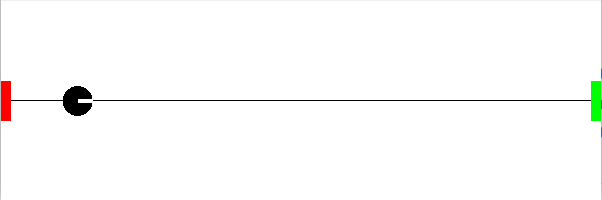
\includegraphics[width=0.3\linewidth]{env/visualizations/1d.png}
  \caption{1 dimensional environment, 2 rewards}
  \label{fig:1d_env}
  \vspace{2cm}
\end{figure}

\begin{figure}[H]
  \centering
    \hspace{2cm}
  \begin{subfigure}[b]{0.3\linewidth}
    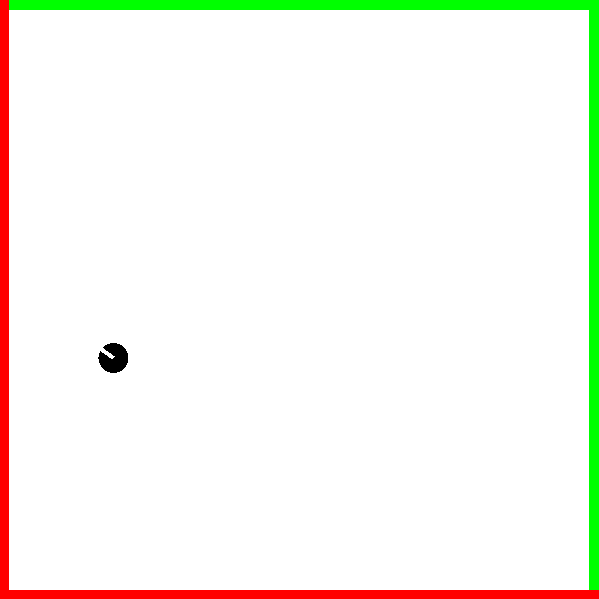
\includegraphics[width=\linewidth]{env/visualizations/2d_2reward.png}
      \caption{2 rewards per dimension}
      \label{fig:2d_2_env}
  \end{subfigure}
    \hspace{2cm}
   \begin{subfigure}[b]{0.3\linewidth}
    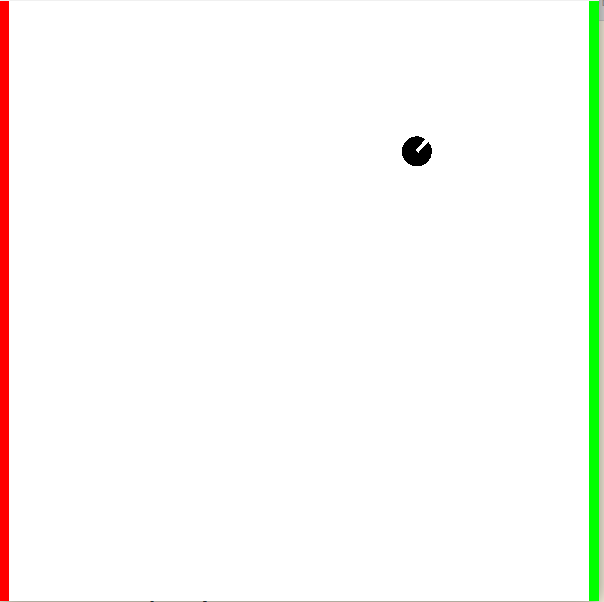
\includegraphics[width=\linewidth]{env/visualizations/2d_1reward.png}
    \caption{2 rewards on the first dimension only}
    \label{fig:2d_1_env}
  \end{subfigure}
  \hspace{2cm}
  \caption{2 dimensional environment with different reward configurations}
  \label{fig:2d_env}
\end{figure}


\section{Algorithm}

We used an implementation of the DDPG algorithm from Scott Fujimoto \cite{fujimoto_pytorch_2019}, while some modifications were applied to add the required functionalities. The core of those algorithms remains as described in the original paper \cite{lillicrap_continuous_2015} that introduced it. DDPG is a model-free deep reinforcement learning algorithm, which runs on continuous environments with continuous controls. It explores the environment and saves all its experiences in a replay buffer. DDPG learns from the content of the replay buffer.

A replay buffer \cite{mnih_playing_2013} is a queue of size $N$ containing experiences. An experience is a tuple $({s}_{t},{a}_{t},{r}_{t},{s}_{t+1})$ where ${s}_{t}$ is a state, ${a}_{t}$ is the action taken in state ${s}_{t}$, ${r}_{t}$ is the reward gained by taking this action on this state, ${s}_{t+1}$ is the state resulting from the action. When the replay buffer is full, the oldest sample are removed and the newest are added.

DDPG is composed of two neural networks, the actor and the critic. The actor is the one which decides the action to perform, according to its observations. It learns by maximizing the output of the critic network. The critic learns the action value by propagating the rewards associated with experiences in the replay buffer.

The implementation is in Python3, using the PyTorch library. The functionalities that we added are related to data extraction and configurability. The first one being $Q(s, \Pi(s))$ allowing us to extract the Critic Q values approximations of the current policy $\Pi(s)$, $s$ being a discretization of the observation space. Since a visualization of the Actor's decision might be useful, we introduced a second functionality computing $\Pi(s)$ to extract and visualize the Actor's decisions over the same discretization of the observation space.

\section{User documentation}

The source code of the project is available on \url{https://github.com/schott97l/RL_analysis}.
The repository contains two independents submodules, \url{https://github.com/schott97l/RL_implementations} and\\ \url{https://github.com/hroussille/RL-evaluation-environment}, and the scripts of the studies.

To run this project, Python3.6 or newer is required with PyTorch, Gym, Numpy, Matplotlib and PyOpenGL:
\begin{lstlisting}
pip install numpy matplotlib torch torchvision pyopengl gym 
\end{lstlisting}

You can download the project and install it by running the following commands:
\begin{lstlisting}
git clone https://github.com/schott97l/RL_analysis.git
cd RL_analysis && git submodule update --init
pip install -e RL-evaluation-environment/gym-hypercube
\end{lstlisting}
\ \\

The command below is used to learn a policy on our hypercube environment:
\begin{lstlisting}
python learn_hypercube.py [parameters]
\end{lstlisting}

parameters:

\def\arraystretch{1.5}%  1 is the default, change whatever you need
\begin{center}
\begin{longtable}{l l l}
    \lstinline|--algorithm=<str>| & name of the algorithm to use, "TD3" or "DDPG" & default="DDPG"\\
    \lstinline|--seed=<int>| & seed for the random exploration & default=random\\
    \lstinline|--dimensions=<int>| & number of dimensions of the environment & default=2"\\
    \lstinline|--eval_freq=<int>| & how often (time steps) we evaluate & default=2e3\\
    \lstinline|--exploration_timesteps=<int>| & exploration duration & default=1e4\\
    \lstinline|--exploration_mode=<str>| & "random\_walk" or "uniform" &  default="random\_walk"\\
    \lstinline|--learning_timesteps=<int>| & learning duration & default=1e4\\
    \lstinline|--buffer_size=<int>| & size of the replay buffer & default=1e4\\
    \lstinline|--no_new_exp| & learn from a fixed batch &\\
    \lstinline|--expl_noise=<float>| & noise & default=0.1\\
    \lstinline|--batch_size=<int>| & learning batch & default=64\\
    \lstinline|--discount=<float>| & discount factor & default=0.99\\
    \lstinline|--actor_hl1=<int>| & actor first hidden layer size & default=40\\
    \lstinline|--actor_hl2=<int>| & actor second hidden layer size & default=30\\
    \lstinline|--critic_hl1=<int>| & critic first hidden layer size & default=40\\
    \lstinline|--critic_hl2=<int>| & critic second hidden layer size & default=30\\
    \lstinline|--learning_rate=<float>| & learning rate of the networks & default=1e-4\\
    \lstinline|--tau=<float>| & target network update rate & default=5e-3\\
    \lstinline|--policy_noise=<float>| & noise added to target policy during critic update & default=0.2\\
    \lstinline|--noise_clip=<float>| & range to clip target policy noise & default=0.5\\
    \lstinline|--policy_freq=<int>| & frequency of delayed policy updates & default=2\\
    \lstinline|--quiet| & to not print on standard output &\\
    \lstinline|--acceleration| & set acceleration mode & default: velocity\\
    \lstinline|--discrete| & set discrete actions & default: continuous\\
    \lstinline|--speed_limit_mode| & set max velocity mode, "vector\_norm" or "independent" & default="vector\_norm"\\
    \lstinline|--replay_buffer_visu| & visualize 2D replay buffer&\\
    \lstinline|--no_policy_visu| & to not plot visualizations&\\
    \lstinline|--no_render| & to not render the environment&\\
    \lstinline|--save| & save logs, models or visualizations&\\
    \lstinline|--output=<str>| & output directory & default="results"\\
    \lstinline|--high_reward_value=<float>| & value of the high reward & default=1\\
    \lstinline|--low_reward_value=<float>| & value of the low reward & default=0.1\\
    \lstinline|--high_reward_count=<str>| & "half" or "one" & default="half"\\
    \lstinline|--low_reward_count=<str>| & "half" or "one" & default="half"\\
    \lstinline|--mode=<str>| & rewards positions "deterministic" or "random" & default="deterministic"\\
    \lstinline|--reset_radius=<float>| & radius from the center for the agent spawn & default=None\\
    \lstinline|--filter| & to add a circle filter of the replay buffer & \\
    \lstinline|--filter_radius=<float>| & radius of the filter & default=0.2\\
    \lstinline|--filter_pos=<float>| & position of the filter on the diagonal of the environment & default=0\\
\end{longtable}
\end{center}

\ \\

The command below is used to run a policy which has been learned with the previous script.
\begin{lstlisting}
python run_hypercube.py [parameters]
\end{lstlisting}

parameters:

\def\arraystretch{1.5}
\begin{center}
\begin{longtable}{l l l}
    \lstinline|--algorithm=<str>| & name of the algorithm to use, "TD3" or "DDPG" & default="DDPG"\\
    \lstinline|--policy_directory=<str>| & & default="results/models"\\
    \lstinline|--dimensions=<int>| & number of dimensions of the environment & default=2"\\
    \lstinline|--max_episodes=<int>| & & default=50\\
    \lstinline|--max_timesteps=<str>| & & default=1e4\\
    \lstinline|--buffer_size=<str>| & size of the replay buffer & default=5e3\\
    \lstinline|--quiet| & to not print on standard output &\\
    \lstinline|--acceleration| & to set acceleration mode, default: velocity\\
    \lstinline|--discrete| & to set discrete actions, default: continuous\\
    \lstinline|--no_render| & to not render the environment\\
    \lstinline|--high_reward_value=<float>| & value of the high reward & default=1\\
    \lstinline|--low_reward_value=<float>| & value of the low reward & default=0.1\\
    \lstinline|--high_reward_count=<str>| & "half" or "one" & default="half"\\
    \lstinline|--low_reward_count=<str>| & "half" or "one" & default="half"\\
    \lstinline|--mode=<str>| & rewards positions "deterministic" or "random" & default="deterministic"\\
    \lstinline|--reset_radius=<float>| & radius from the center for the agent spawn & default=None\\
\end{longtable}
\end{center}

\section{Studies}

\subsection{Theoretical modeling}

Before analysing any experimental result on the 2D environment, we first decided to calculate the theoretical optimal value and policy by discretizing the environment in order to perform the value iteration algorithm on it \cite{bellman_markovian_1957}. We discretized the 2D environment in a 80x80 grid.

\begin{figure}[H]
  \centering
  \begin{subfigure}[b]{0.45\linewidth}
    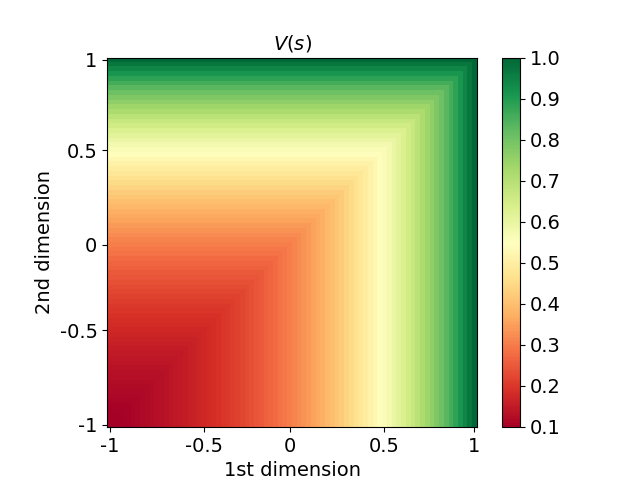
\includegraphics[width=\linewidth]{discrete/discrete_contour.png}
    \caption{Theoretical optimal value: $V(s)$ }
  \end{subfigure}
  \begin{subfigure}[b]{0.45\linewidth}
    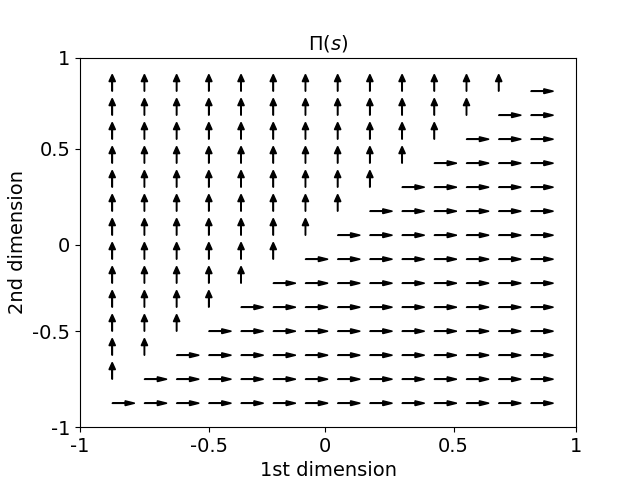
\includegraphics[width=\linewidth]{discrete/discrete_arrow.png}
      \caption{Theoretical optimal policy: $\Pi(s)$ }
  \end{subfigure}
  \caption{Theoretical optimal policy obtained by policy iteration}
  \label{fig:theoretical_policy}
\end{figure}

Figure \ref{fig:theoretical_policy} show us the visualization of the optimal state value and the associated policy. We can see that the more we are close to the right or top edge greater the state value is, and the optimal policy involved is to go straight to right or top edge (the closest) to get the maximum reward.

\subsection{Experimental methodology}

All the presented results are the results of 8 experiments obtained by running the training with exactly the same parameters. The curves and the errors bars shown are the average and the standard deviation over these 8 experiments. The parameters used for each study are specified before, the non specified ones are set to their default value as described in the user documentation.

\subsection{Study 1: Size of the replay buffer}

According to \cite{fujimoto_off-policy_2018} a drawback of DDPG is that it has trouble learning from a fixed batch of experiences in a replay buffer without having the possibility to add new experiences in this replay buffer. So in this study we analyze the influence of the size of a fixed batch of experiences in a replay buffer on the average score of DDPG.

This study runs with the batch learning method, this means that the replay buffer is filled before the beginning of the training and DDPG is not allowed to push any new experience into the replay buffer, making the exploration phase the only source of information on the environment. So it is important to choose how to proceed to this exploration. We decided to test the two common ways to do this, the first one, uniform exploration consists in drawing an initial state from a uniform distribution, then an action is sampled from another uniform distribution over the action space. The full experience is then created when applying the sampled action on the initial state. At each iteration, the whole process restarts. The second exploration scheme is a random walk where an initial state and an action are sampled as in the uniform exploration. However, any subsequent step will have the previous resulting state in place of its initial state.

For this study we train DDPG for 100k timesteps, with a replay buffer size ranging from ${2}^{4}$ to ${2}^{16}$. The environment is 2 dimensional with high rewards present on the top and right edges and low rewards on the opposite sides.

We expect to see poor performance on the lower replay buffers sizes, as the number of experiences that can be contained in the replay buffer is too low, leading to an almost certain auto correlation of the experiences when sampling from the replay buffer. As the replay buffer size increases, the performance should rise and settle to a level dependent upon the environment. In our 2D environment, the starting position greatly influences the outcome and therefore the average reward obtained. We forced the starting point to be uniformly generated around the center point of the environment in a hyper sphere with a radius of 0.1 in order to reduce the variance that would otherwise be induced.


\subsubsection{Uniform sampled replay buffer}

\begin{figure}[H]
  \centering
  \begin{subfigure}[b]{0.3\linewidth}
    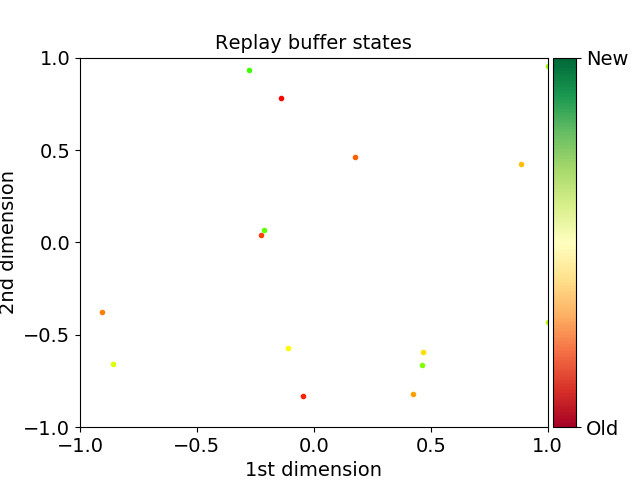
\includegraphics[width=\linewidth]{Study_1/buffer/uniform_16.png}
    \caption{Size 16}
  \end{subfigure}
  \begin{subfigure}[b]{0.3\linewidth}
    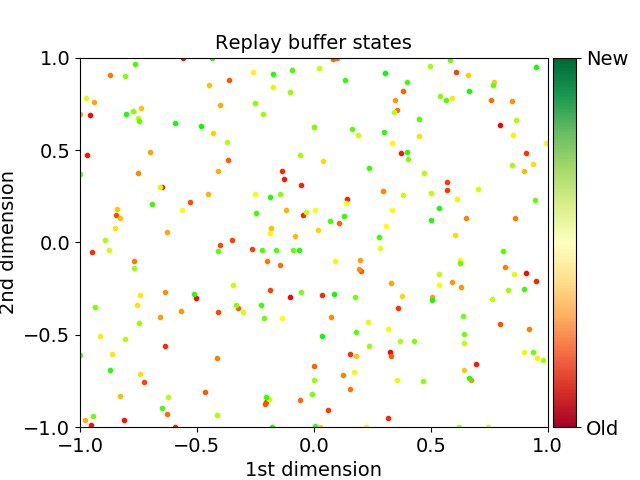
\includegraphics[width=\linewidth]{Study_1/buffer/uniform_256.png}
      \caption{Size 256}
  \end{subfigure}
   \begin{subfigure}[b]{0.3\linewidth}
    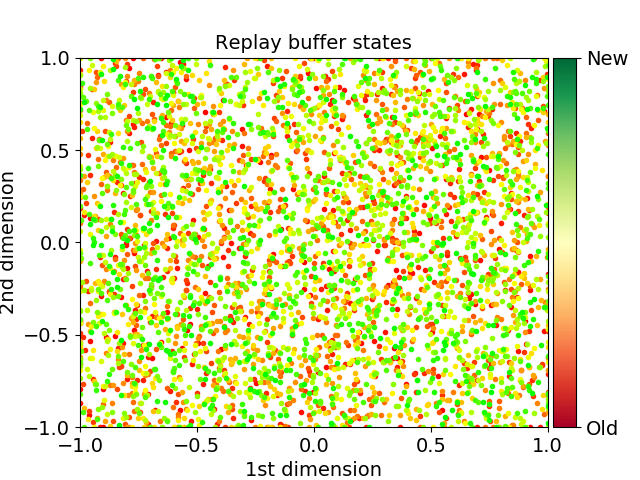
\includegraphics[width=\linewidth]{Study_1/buffer/uniform_4096.png}
    \caption{Size 4096}
  \end{subfigure}
  \caption{Uniform sampled replay buffers}
  \label{fig:buffers_uniform}
\end{figure}

Figure \ref{fig:buffers_uniform} represents replay buffers examples of our 2D environment \ref{fig:2d_2_env}. The visualisations shows the initial position for each experience contained, and the color from red to green means from the oldest to newest experience, this information is not important for a replay buffer filled by uniform exploration, however for replay buffers filled with random walk it allow us to visualize the path taken by the agent during the exploration phase.

Parameters for this experiment:
\begin{itemize}
    \item[] \lstinline|--learning_timesteps=100k|
    \item[] \lstinline|--eval_freq=5k|
    \item[] \lstinline|--exploration_mode="uniform"|
    \item[] \lstinline|--buffer_size=| $2^3, 2^4, 2^6, 2^8, 2^{10}, 2^{12}, 2^{14}$
    \item[] \lstinline|--exploration_timesteps=| $2^3, 2^4, 2^6, 2^8, 2^{10}, 2^{12}, 2^{14}$
\end{itemize}

\begin{figure}[H]
  \centering
    \begin{subfigure}[b]{0.45\linewidth}
    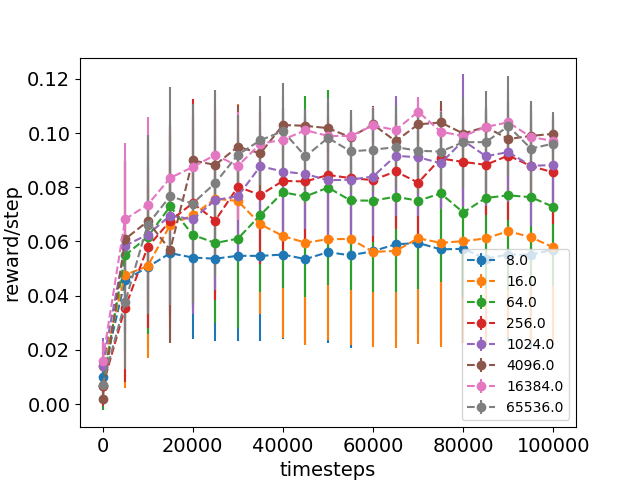
\includegraphics[width=\linewidth]{Study_1/1.1/curves1_1.png}
    \caption{Scores for each replay buffer size}
    \end{subfigure}
    \begin{subfigure}[b]{0.45\linewidth}
    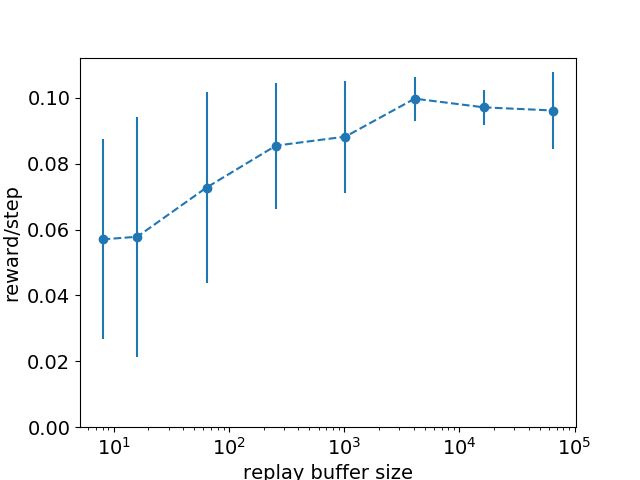
\includegraphics[width=\linewidth]{Study_1/1.1/total_scores1_1.png}
    \caption{Final scores according to the replay buffer size}
    \end{subfigure}
    \caption{Uniform sampling}
  \label{fig:scores_uniform}
\end{figure}

Figure \ref{fig:scores_uniform} shows the score reached by DDPG for each replay buffer size, as we can see, the score seems to be converging quite early. With replay buffers of size 256 and more, 100k learning steps are enough to converge close to the optimal policy. We can observe that bigger replay buffers does not necessarily imply better scoring performances. It can be explained by the uniform character of the sampling. However even if DDPG can converge with small replay buffers, we can also observe that the standard deviation reduces when the size of the replay buffer increases. It can be because with too few examples a uniform sampling cannot draw a set of positions that is enough representative of the environment. For example in Figure \ref{fig:buffers_uniform} (a) we can see that with a replay buffer of size 16, there was no experience in the top left corner.

\begin{figure}[H]
  \centering
   \begin{subfigure}[b]{0.45\linewidth}
    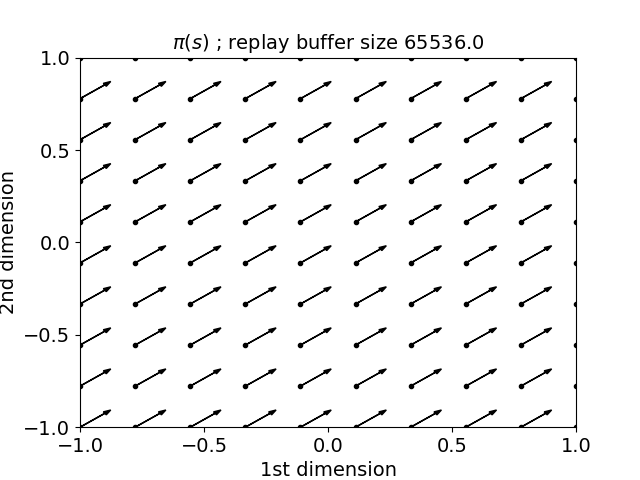
\includegraphics[width=\linewidth]{Study_1/policy/Pi_arrow_65536.png}
      \caption{Policy given by the Actor network}
  \end{subfigure}
  \begin{subfigure}[b]{0.45\linewidth}
    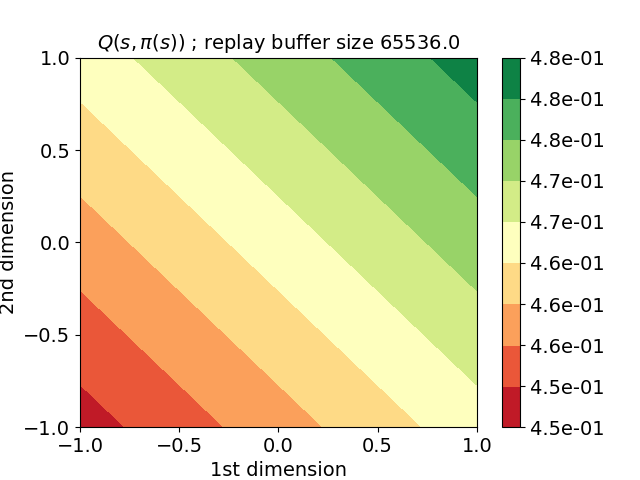
\includegraphics[width=\linewidth]{Study_1/policy/Q_contour_65536.png}
    \caption{Action value given by the Critic for the Actor policy}
  \end{subfigure}
  \caption{Optimal Actor Critic output for a 64k replay buffer}
  \label{fig:64k_policy}
\end{figure}

Figure \ref{fig:64k_policy} show us the optimal policy and the associated action value learned by DDPG after 100k learning timesteps on a 64k replay buffer. We can see that the policy and the action value learned by DDPG are different from the theoretical ones \ref{fig:theoretical_policy}. Even if the policy is similar to the theoretical policy by going to the top right corner, we can see that DDPG did not learn that going straight towards the closest edge will allow to get the reward quicker that moving in diagonal. We can also notice that the action value learned by DDPG is a kind of linear regression of the action value calculated by value iteration in the discretized environment, and the policy learned by DDPG seems to follow this linear regression, that's probably why it move to the top right corner diagonally.

Trying to investigate on this difference we tried several set of parameters with learning timesteps ranging from 10K to 1M and changing the activation functions of the actor and critic networks from ReLu to Tanh. More can be done but our results tend to show that DDPG is unable to correctly approximate the real Q value function.


\subsubsection{Random walk explored replay buffer}

We saw with the previous study that even with a very small replay buffer, DDPG can converge in our 2D environment \ref{fig:2d_2_env}. And this is probably possible because the environment is very basic and because the sampling of the replay buffer is uniform. In this study we will look at whether DDPG can converge on our 2D environment with small replay buffer, when replay buffer aren't sampled uniformly but filled with a random walk exploration. So the parameters of the experiment are the sames as the previous one, except how to fill the buffer.

Parameters for this experiment:
\begin{itemize}
    \item[] \lstinline|--learning_timesteps=100k|
    \item[] \lstinline|--eval_freq=5k|
    \item[] \lstinline|--exploration_mode="random_walk"|
    \item[] \lstinline|--buffer_size=| $2^3, 2^4, 2^6, 2^8, 2^{10}$
    \item[] \lstinline|--exploration_timesteps=| $2^3, 2^4, 2^6, 2^8, 2^{10}$
\end{itemize}

\begin{figure}[H]
    \begin{subfigure}[b]{0.3\linewidth}
    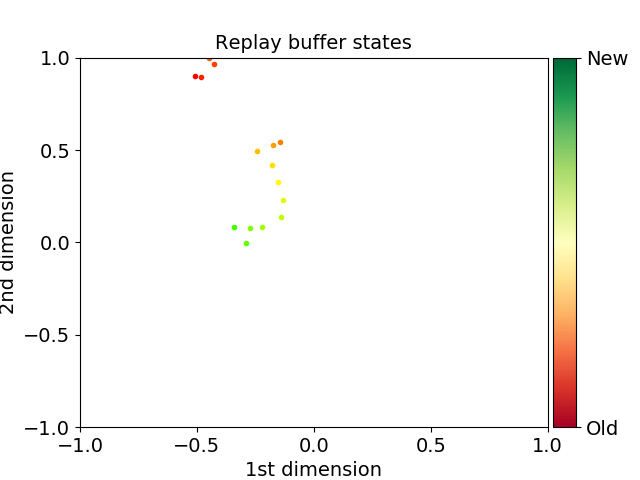
\includegraphics[width=\linewidth]{Study_1/buffer/sequential_16.png}
    \caption{Size 16}
  \end{subfigure}
  \begin{subfigure}[b]{0.3\linewidth}
    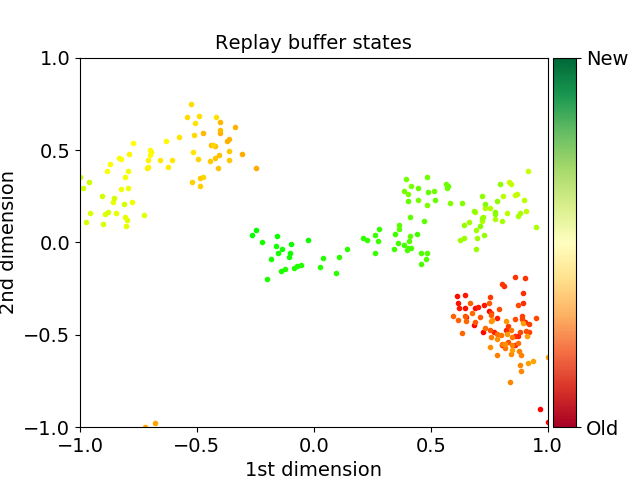
\includegraphics[width=\linewidth]{Study_1/buffer/sequential_256.png}
      \caption{Size 256}
  \end{subfigure}
   \begin{subfigure}[b]{0.3\linewidth}
    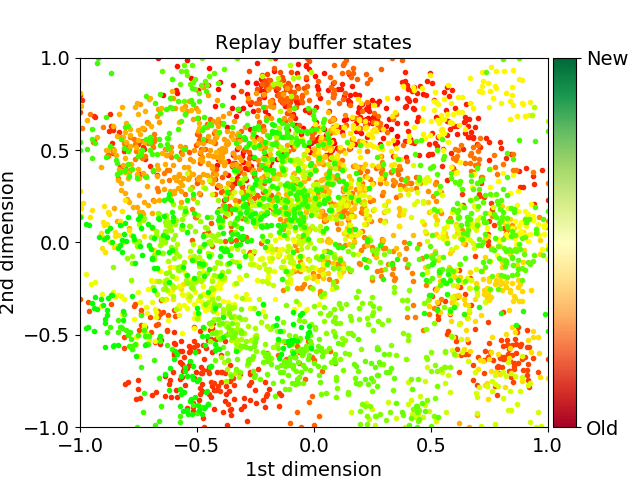
\includegraphics[width=\linewidth]{Study_1/buffer/sequential_4096.png}
    \caption{Size 4096}
  \end{subfigure}
  \caption{Random walk replay buffer}
  \label{fig:buffers_random_walk}
\end{figure}

Figure \ref{fig:buffers_random_walk} shows replay buffer filled by random walk exploration. And on the contrary to the uniform sampling techniques, this one does not cover the entire space of the environment when replay buffer are too small. But with big replay buffers, the two techniques tend to give the same results. So by running DDPG on these replay buffer we expect that small replay buffers give a very bad results, but bigger the replay buffer will be much more the results should approach the results of replay buffer uniformly sampled.

\begin{figure}[H]
  \centering
    \begin{subfigure}[b]{0.45\linewidth}
    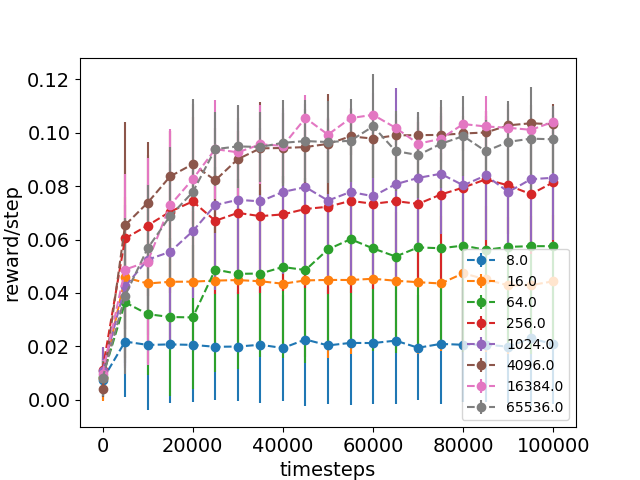
\includegraphics[width=\linewidth]{Study_1/1.2/curves1_2.png}
    \caption{Scores for each replay buffer size}
    \end{subfigure}
    \begin{subfigure}[b]{0.45\linewidth}
    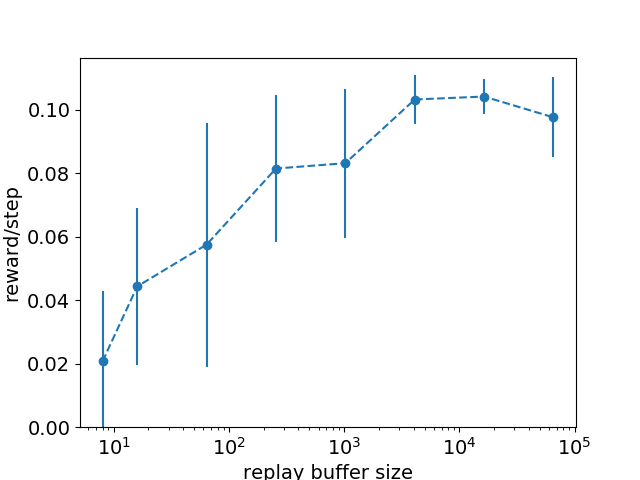
\includegraphics[width=\linewidth]{Study_1/1.2/total_scores1_2.png}
    \caption{Final scores according to the replay buffer size}
    \end{subfigure}
    \caption{Random walk exploration}
  \label{fig:scores_random_walk}
\end{figure}

On the contrary to the study with uniform sampling, here there is a significant increase of the score according to the replay buffer size. So it confirms our expectations, small replay buffer (here under 1024 replays) seems to be insufficient for DDPG to learn. And this is probably because the agent has not enough timesteps to discover the entire environment, it only knows the region it appeared so it cannot know where rewards are. As seen in Figure \ref{fig:scores_random_walk} above, under the size of 256, experiences achieved very poor performances moreover their respective standard deviation are far superior to any other run with bigger replay buffer, which suggest that barely no information could be learned from the environment with so small replay buffer and random walk exploration. On the other hand, the bigger replay buffer allowed DDPG to converge close to the optimal policy as expected. An interesting note is that we can see no significant difference between the 1024 long replay buffer and the sizes above, this result might be explained by the simplicity of the environment.


\subsection{Study 2: Filtered replay buffer}

In this study, we analyse the influence of a filtered replay buffer on the performances of DDPG on a 2 dimensional environment in order to test the limits of function approximators  in different environment configurations \cite{schaul_universal_2015}. The filter imposes a circular unexplored region in the environment. The flag $--no_new_exp$ is set for the whole study.

Several configurations are studied, where we act on the filter position and size while using different exploration schemes. For each of them the learning timesteps parameter is set to 100k, on a replay buffer that can contain up to 4096 steps.

The environment being 2 dimensional where each dimension $d\in[-1,1]$, we can visualize the content of a replay buffer to see the explored regions with the different exploration schemes and filter positions.

\begin{figure}[H]
  \centering
  \begin{subfigure}[b]{0.3\linewidth}
    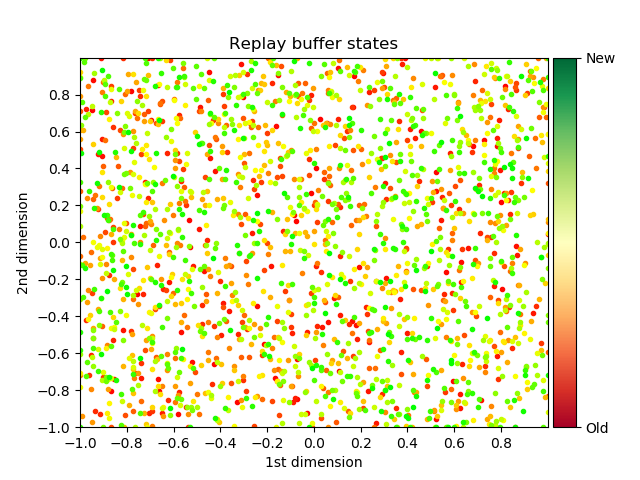
\includegraphics[width=\linewidth]{Study_2/visualizations/uniform.png}
    \caption{Uniform unfiltered}
  \end{subfigure}
  \begin{subfigure}[b]{0.3\linewidth}
    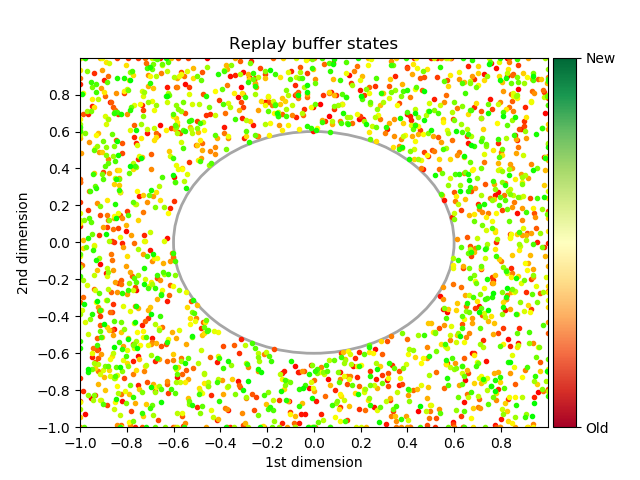
\includegraphics[width=\linewidth]{Study_2/2.1/visualizations/uniform-center.png}
      \caption{Uniform center filtered}
  \end{subfigure}
   \begin{subfigure}[b]{0.3\linewidth}
    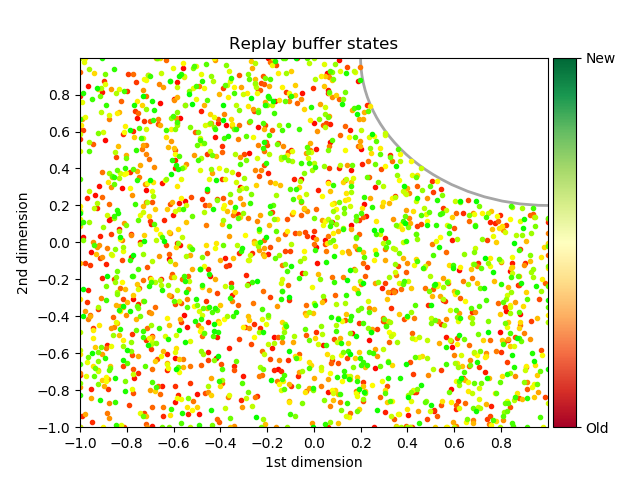
\includegraphics[width=\linewidth]{Study_2/2.3/visualizations/uniform-corner.png}
    \caption{Uniform corner filtered}
  \end{subfigure}
    \begin{subfigure}[b]{0.3\linewidth}
    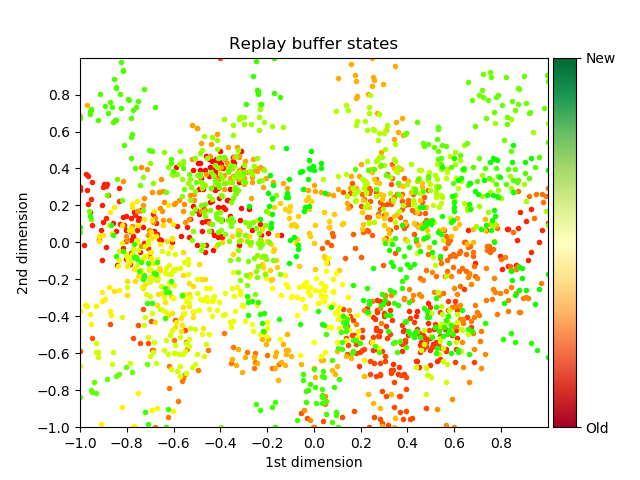
\includegraphics[width=\linewidth]{Study_2/visualizations/sequential.png}
    \caption{Random walk unfiltered}
  \end{subfigure}
  \begin{subfigure}[b]{0.3\linewidth}
    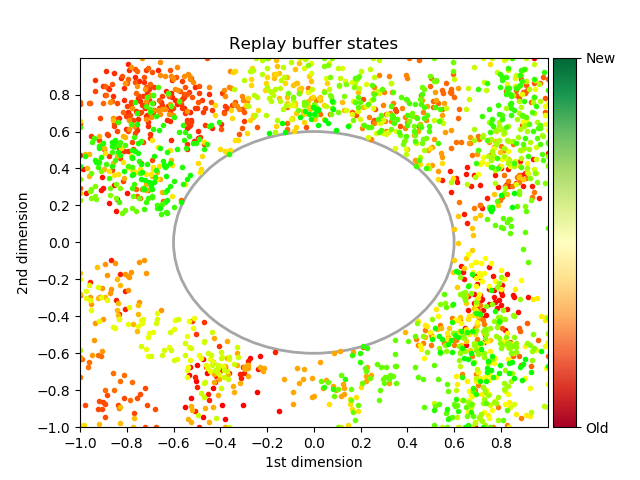
\includegraphics[width=\linewidth]{Study_2/2.2/visualizations/sequential-center.png}
      \caption{Random walk center filtered}
  \end{subfigure}
   \begin{subfigure}[b]{0.3\linewidth}
    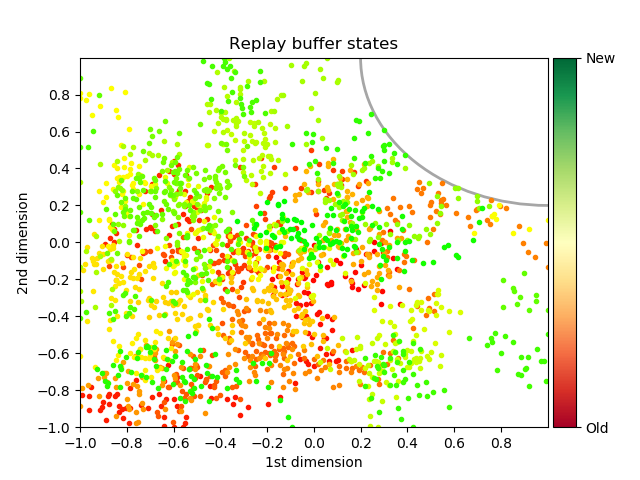
\includegraphics[width=\linewidth]{Study_2/2.4/visualizations/sequential-corner.png}
    \caption{Random walk corner filtered}
  \end{subfigure}
  \label{fig:filter_random_walk}
   \caption{Sample filtered replay buffers}
\end{figure}

The exploration mode should play a critical role in the convergence rate, as the random walk exploration will explore a smaller portion of the environment than the uniform one on average. This phenomenon is more apparent as fewer experiences are sampled. Intuitively, the size of the filter should also influence the performance as DDPG will be required to interpolate or extrapolate (depending on the filter position) in order to converge to the optimal policy.

The filter that we use is circular, with $\theta$ the center of the filter, $r$ its radius and $x$ a point in the n dimensional space the indicator function that we use to know if a point is in the filter is:

\begin{equation}
\mathbbm{1}_F(x) := 
    \begin{cases}
      1,\:if\:\sqrt(\sum\limits_{i=1}^n (\theta_i - x_i) ^ 2)\:<\:r\\
      0,\:otherwise.
      \end{cases}
\end{equation}
 
 Therefore, we do allow points that are lying on the filter boundary.
 
We will compare the resulting policies to the optimal policy shown in Figure \ref{fig:theoretical_policy} and evaluate how the learned policy deviates from it for several key size and positions of filter.

\subsubsection{Uniform exploration and centered filter}

This study focuses on the behaviour of DDPG on a replay buffer with uniform exploration and a  center filter with a radius ranging from 0 (no filter) to 1.2

Parameters for this experiment:
\begin{itemize}
    \item[] \lstinline|--learning_timesteps=100k|
    \item[] \lstinline|--eval_freq=5k|
    \item[] \lstinline|--exploration_mode="uniform"|
    \item[] \lstinline|--buffer_size=4096|
    \item[] \lstinline|--exploration_timesteps=4096|
    \item[] \lstinline|--filter_position=0|
    \item[] \lstinline|--filter_size=0, 0.2, 0.4, 0.6, 0.8, 1, 1.2|
\end{itemize}

\begin{figure}[H]
  \centering
   \begin{subfigure}[b]{0.4\linewidth}
    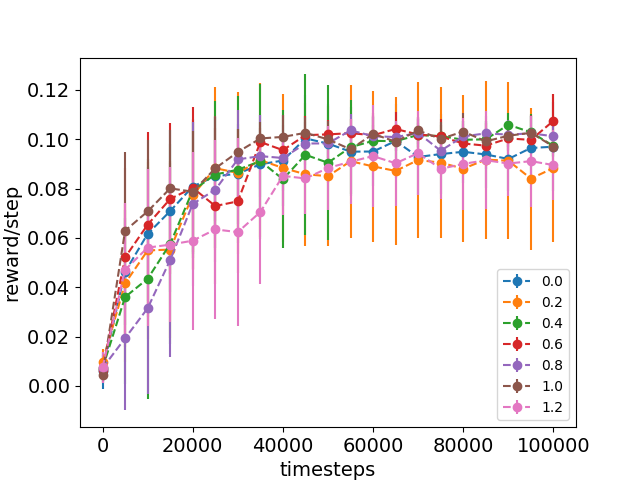
\includegraphics[width=\linewidth]{Study_2/2.1/visualizations/scores_filter_size.png}
      \caption{Learning curves for each size of filter}
  \end{subfigure}
  \begin{subfigure}[b]{0.4\linewidth}
    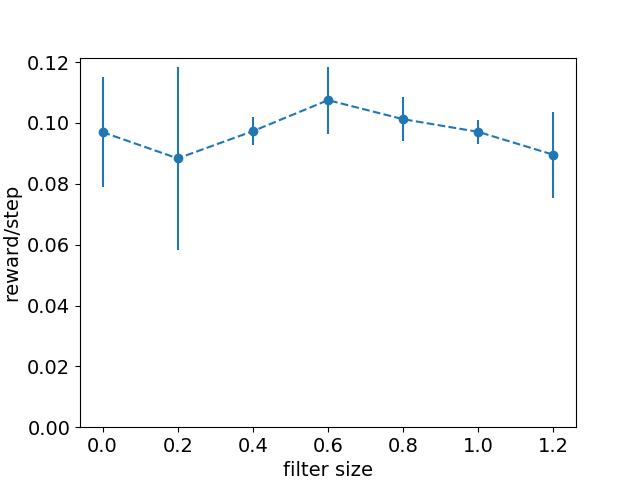
\includegraphics[width=\linewidth]{Study_2/2.1/visualizations/total_scores.png}
    \caption{final score according to the filter size}
  \end{subfigure}
   \caption{center filter with uniform exploration}
   \label{fig:center_curves_uniform}
\end{figure}

In Figure \ref{fig:center_curves_uniform} we cannot see any significant difference on the performance achieved according to the filter size. It is however important to present the resulting $Q(s, \Pi(s))$ for some filter size value to understand how DDPG adapted to the presence of the filter. Please note that the $\Pi(s)$ visualizations are not included as they were all optimal.

\begin{figure}[H]
  \centering
   \begin{subfigure}[b]{0.3\linewidth}
    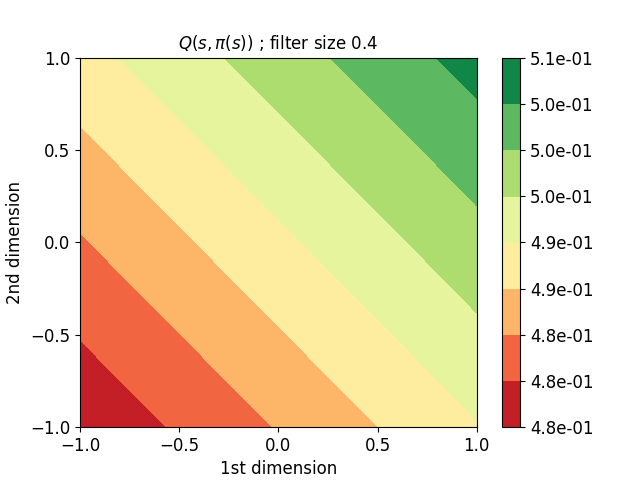
\includegraphics[width=\linewidth]{Study_2/2.1/visualizations/Q_contour_0_4.png}
      \caption{0.4 radius $Q(s, \Pi(s))$}
  \end{subfigure}
   \begin{subfigure}[b]{0.3\linewidth}
    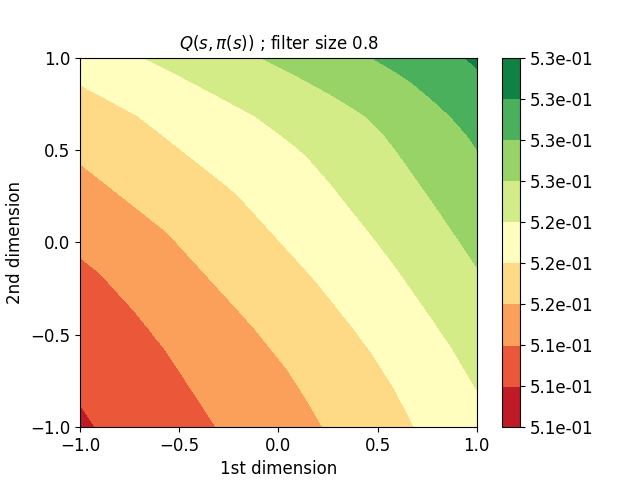
\includegraphics[width=\linewidth]{Study_2/2.1/visualizations/Q_contour_0_8.png}
      \caption{0.8 radius $Q(s, \Pi(s))$}
  \end{subfigure}
   \begin{subfigure}[b]{0.3\linewidth}
    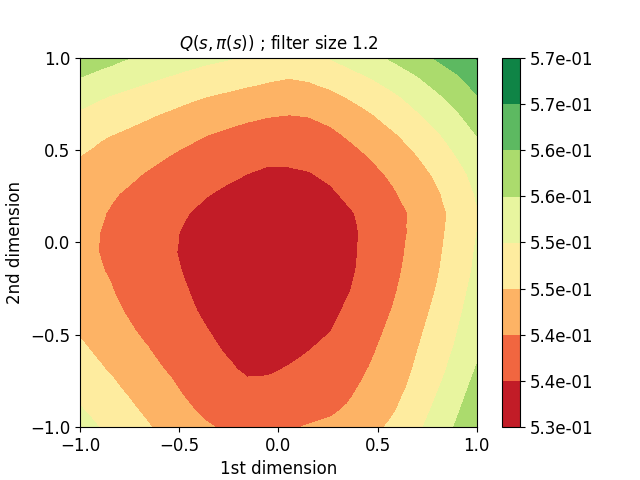
\includegraphics[width=\linewidth]{Study_2/2.1/visualizations/Q_contour_1_2.png}
      \caption{1.2 radius $Q(s, \Pi(s))$}
  \end{subfigure}
   \caption{Sample policies: center filter with uniform exploration}
    \label{fig:center_contour_uniform}
\end{figure}

DDPG with a uniform exploration is able to converge even when a significant proportion of the environment is left unexplored due to a centered filter.
The estimated Q values seem to increase proportionally to the filter size, but there is no evidence to conclude that a divergent behaviour took place during the learning process.

We can clearly see that the centered filter had an effect on the learned policy in Figure \ref{fig:center_contour_uniform} by comparing this result with Figure \ref{fig:64k_policy} but this effect did not impact the performance. Mostly because of the simplicity of the environment and the independence of each dimensions with respect to the others.

\subsubsection{Random walk exploration and centered filter}

This study focuses on the behaviour of DDPG on a replay buffer with random walk exploration and a  center filter with a radius ranging from 0 (no filter) to 1.2

Parameters for this experiment:
\begin{itemize}
    \item[] \lstinline|--learning_timesteps=100k|
    \item[] \lstinline|--eval_freq=5k|
    \item[] \lstinline|--exploration_mode="random_walk"|
    \item[] \lstinline|--buffer_size=4096|
    \item[] \lstinline|--exploration_timesteps=4096|
    \item[] \lstinline|--filter_position=0|
    \item[] \lstinline|--filter_size=0, 0.2, 0.4, 0.6, 0.8, 1, 1.2|
\end{itemize}

\begin{figure}[H]
  \centering
   \begin{subfigure}[b]{0.4\linewidth}
    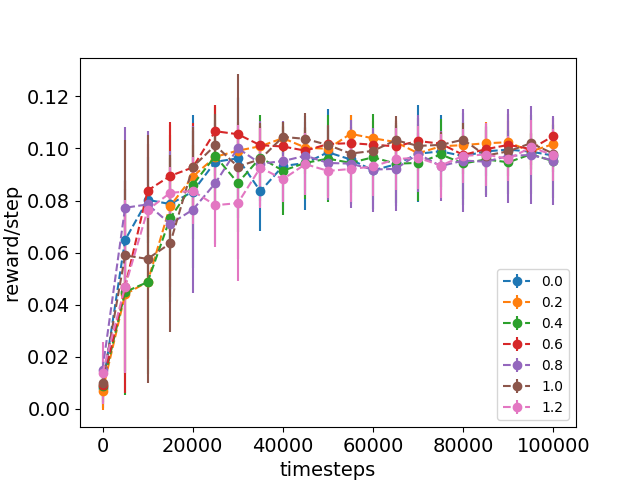
\includegraphics[width=\linewidth]{Study_2/2.2/visualizations/scores_filter_size.png}
      \caption{Learning curves for each size of filter}
  \end{subfigure}
  \begin{subfigure}[b]{0.4\linewidth}
    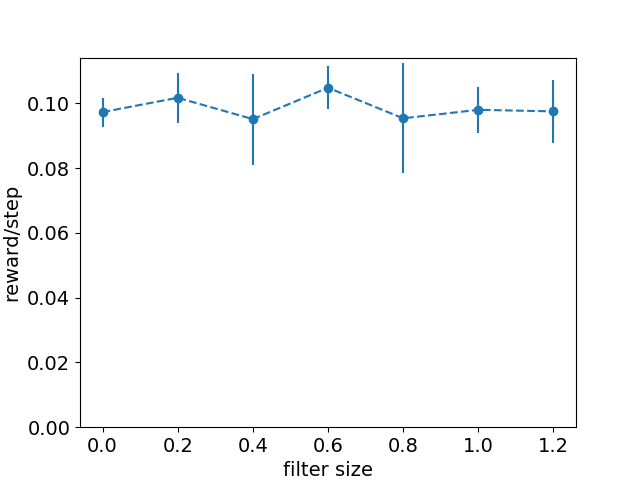
\includegraphics[width=\linewidth]{Study_2/2.2/visualizations/total_scores.png}
    \caption{Final score according to the filter size}
  \end{subfigure}
   \caption{Center filter with random walk exploration}
   \label{fig:center_curves_random_walk}
\end{figure}

The result are very similar to the previous case where no significant performance drop can be observed in Figure \ref{fig:center_curves_random_walk}.

\begin{figure}[H]
  \centering
   \begin{subfigure}[b]{0.3\linewidth}
    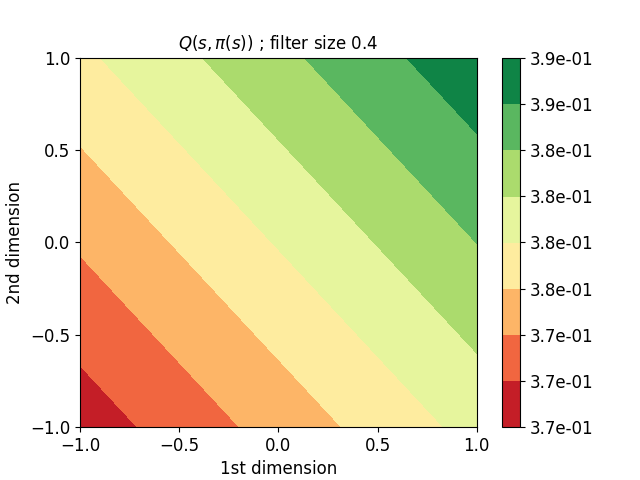
\includegraphics[width=\linewidth]{Study_2/2.2/visualizations/Q_contour_0_4.png}
      \caption{0.4 radius $Q(s, \Pi(s))$}
  \end{subfigure}
   \begin{subfigure}[b]{0.3\linewidth}
    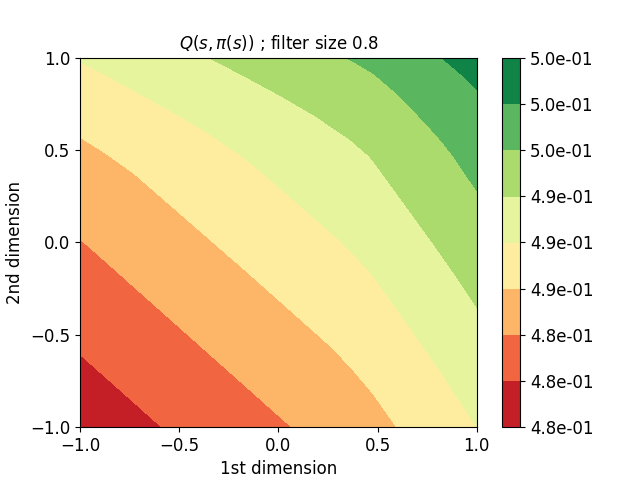
\includegraphics[width=\linewidth]{Study_2/2.2/visualizations/Q_contour_0_8.png}
      \caption{0.8 radius $Q(s, \Pi(s))$}
  \end{subfigure}
   \begin{subfigure}[b]{0.3\linewidth}
    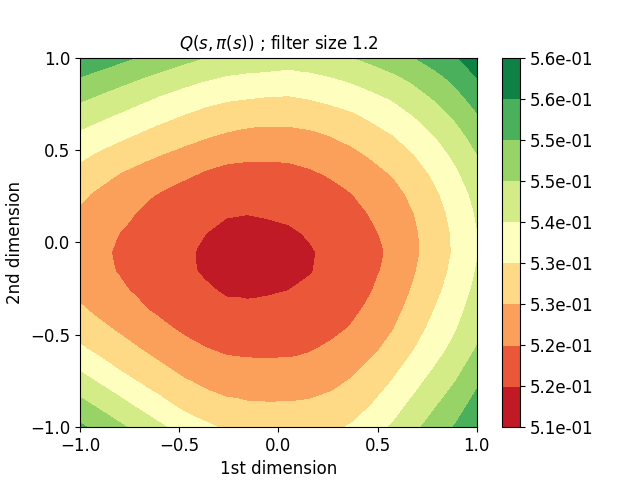
\includegraphics[width=\linewidth]{Study_2/2.2/visualizations/Q_contour_1_2.png}
      \caption{1.2 radius $Q(s, \Pi(s))$}
  \end{subfigure}
   \caption{Sample policies : center filter with random walk exploration}
    \label{fig:center_contour_random_walk}
\end{figure}

Figure \ref{fig:center_contour_random_walk} show us the resulting $Q(s, \Pi(s))$ for the same sample filter size value. Almost no difference with the uniform exploration can be observed as the number of experiences is above the threshold seen in study 1.

\subsubsection{Uniform exploration and cornered filter}

This study focuses on the behaviour of DDPG on a replay buffer with uniform exploration and a filter in the top right corner with a radius ranging from 0 (no filter) to 2.2. As the filter is now in the corner covering the most rewarding spot in the environment one could expect a drop in performance proportional to the filter size since it will mask a significant proportion of high rewarding positions to DDPG.

Parameters for this experiment:
\begin{itemize}
    \item[] \lstinline|--learning_timesteps=100k|
    \item[] \lstinline|--eval_freq=5k|
    \item[] \lstinline|--exploration_mode="uniform"|
    \item[] \lstinline|--buffer_size=4096|
    \item[] \lstinline|--exploration_timesteps=4096|
    \item[] \lstinline|--filter_position=1|
    \item[] \lstinline|--filter_size=0.4, 0.8, 1.2, 1.6, 2, 2.2|
\end{itemize}

\begin{figure}[H]
  \centering
   \begin{subfigure}[b]{0.4\linewidth}
    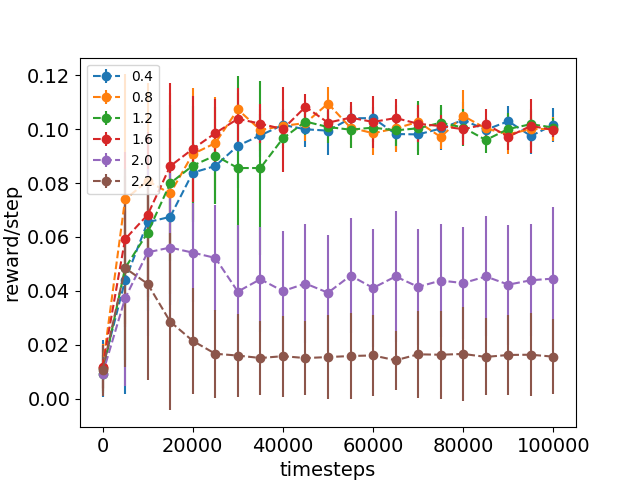
\includegraphics[width=\linewidth]{Study_2/2.3/visualizations/scores_filter_size.png}
      \caption{Learning curves for each size of filter}
  \end{subfigure}
  \begin{subfigure}[b]{0.4\linewidth}
    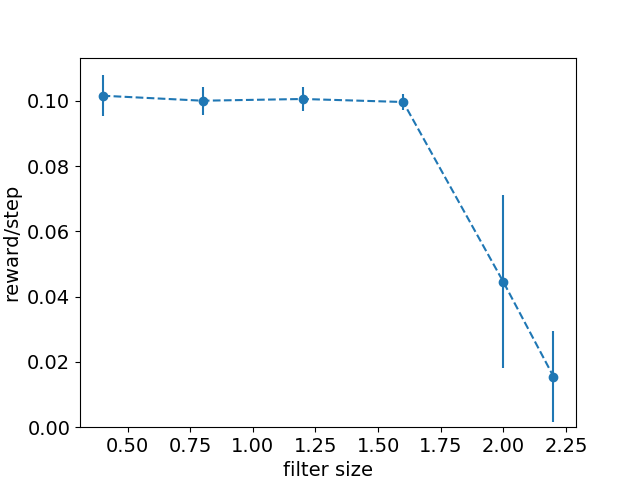
\includegraphics[width=\linewidth]{Study_2/2.3/visualizations/total_scores.png}
    \caption{final score according to the filter size}
  \end{subfigure}
   \caption{corner filter with uniform exploration}
    \label{fig:corner_curves_uniform}
\end{figure}

We can observe the expected performance drop in Figure \ref{fig:corner_curves_uniform} when the filter size exceeds 2.0 while the sizes below do not seem to affect the performance in any significant way.

\begin{figure}[H]
  \centering
   \begin{subfigure}[b]{0.3\linewidth}
    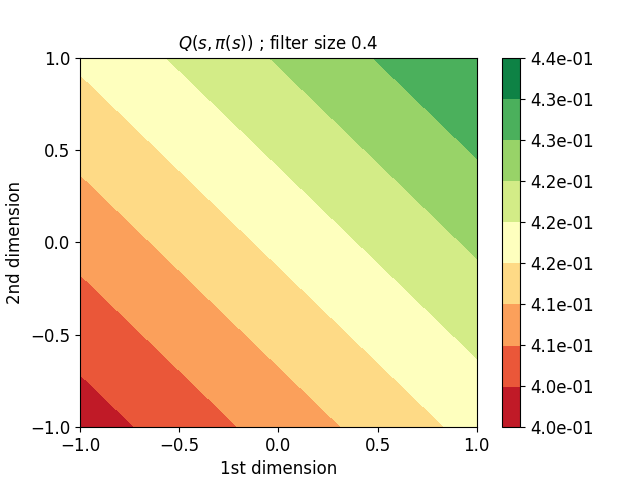
\includegraphics[width=\linewidth]{Study_2/2.3/visualizations/Q_contour_0_4.png}
      \caption{0.4 radius $Q(s, \Pi(s))$}
  \end{subfigure}
   \begin{subfigure}[b]{0.3\linewidth}
    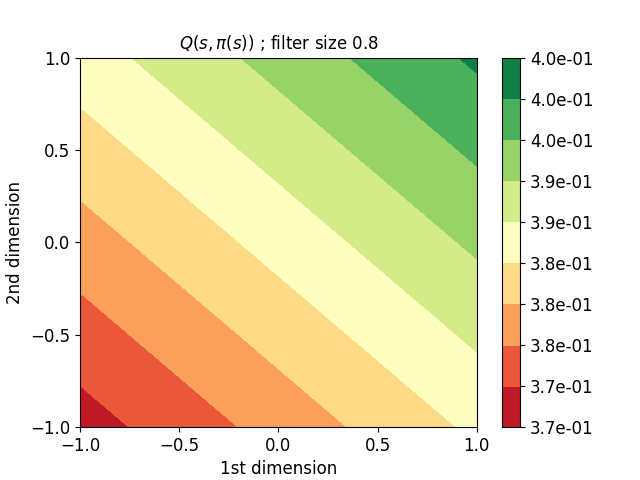
\includegraphics[width=\linewidth]{Study_2/2.3/visualizations/Q_contour_0_8.png}
      \caption{0.8 radius $Q(s, \Pi(s))$}
  \end{subfigure}
   \begin{subfigure}[b]{0.3\linewidth}
    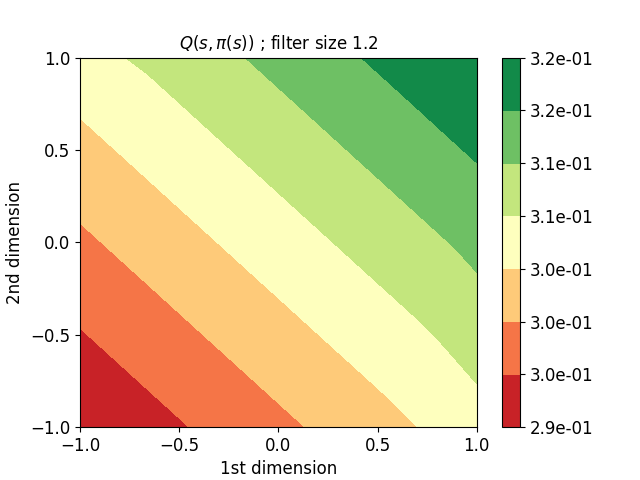
\includegraphics[width=\linewidth]{Study_2/2.3/visualizations/Q_contour_1_2.png}
      \caption{1.2 radius $Q(s, \Pi(s))$}
  \end{subfigure}
   \begin{subfigure}[b]{0.3\linewidth}
    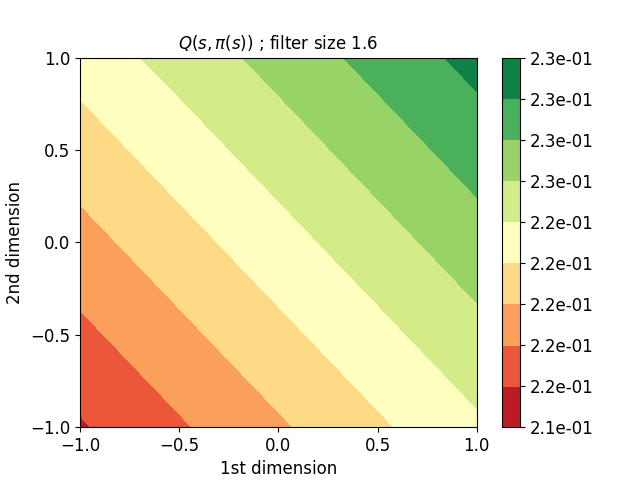
\includegraphics[width=\linewidth]{Study_2/2.3/visualizations/Q_contour_1_6.png}
      \caption{1.6 radius $Q(s, \Pi(s))$}
  \end{subfigure}
   \begin{subfigure}[b]{0.3\linewidth}
    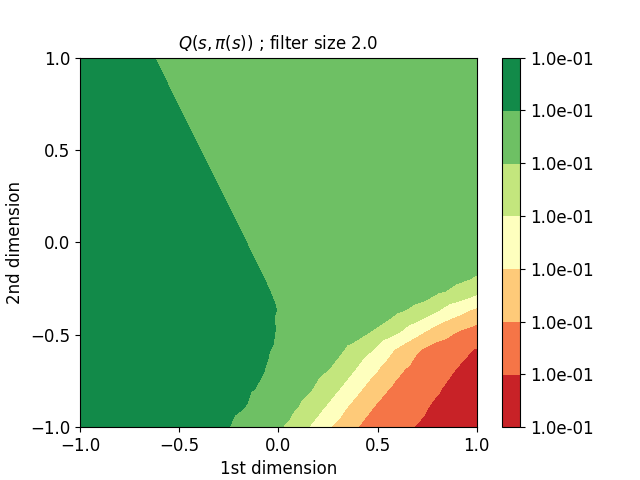
\includegraphics[width=\linewidth]{Study_2/2.3/visualizations/Q_contour_2_0.png}
      \caption{2.0 radius $Q(s, \Pi(s))$}
  \end{subfigure}
    \begin{subfigure}[b]{0.3\linewidth}
    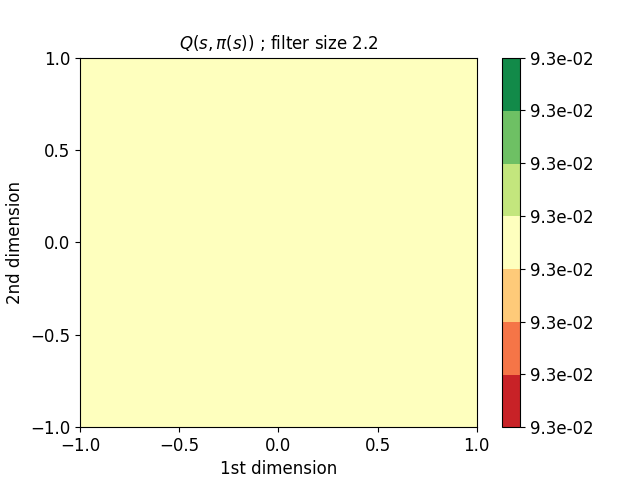
\includegraphics[width=\linewidth]{Study_2/2.3/visualizations/Q_contour_2_2.png}
      \caption{2.2 radius $Q(s, \Pi(s))$}
  \end{subfigure}
   \caption{Sample policies : corner filter with uniform exploration}
   \label{fig:corner_contour_uniform}
\end{figure}

In Figure \ref{fig:corner_contour_uniform} we have the resulting $Q(s, \Pi(s))$ for each filter size value. As we can see, until the filter reaches a critical size of 2.0, masking all dimensions boundaries that would lead to a high reward the Q values estimation are coherent with what was previously observed. 

When the filter radius goes above the 2.0 threshold we do notify that the Q values estimations tends toward 0 over the observations space. The performance drop at this point is significant since the actor is only going on the bottom left corner where the only alternative is a low reward.

Here are the gradient field visualizations of the actor's decisions for the 2.0 and 2.2

\begin{figure}[H]
  \centering
  \hspace{1cm}
   \begin{subfigure}[b]{0.35\linewidth}
    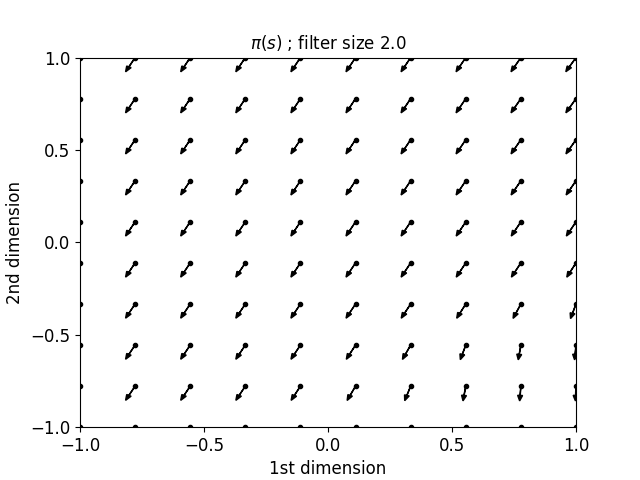
\includegraphics[width=\linewidth]{Study_2/2.3/visualizations/Pi_arrow_2_0.png}
      \caption{2.0 radius $\Pi(s)$}
  \end{subfigure}
  \hspace{1cm}
   \begin{subfigure}[b]{0.35\linewidth}
    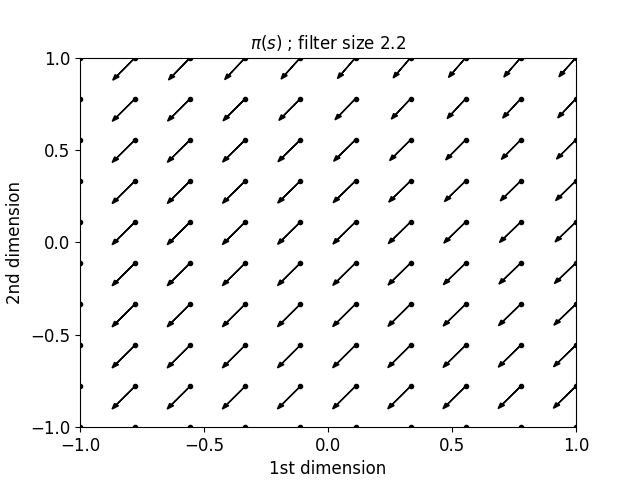
\includegraphics[width=\linewidth]{Study_2/2.3/visualizations/Pi_arrow_2_2.png}
      \caption{2.2 radius $\Pi(s)$}
  \end{subfigure}
  \hspace{1cm}
  \caption{Sample policies : 2.0 and 2.2 radius}
  \label{samples_policies_uniform_corner}
  \end{figure}

It now becomes clear with Figure \ref{samples_policies_uniform_corner} why the 2.0 and 2.2 radius filters have such different impact on the performance. The 2.2 filter radius with no high reward samples forced DDPG to act uniformly in order to reach the bottom left corner where nothing but a low reward is present.

It would seem that DDPG is not able to extrapolate as well as it can interpolate Q values estimations over the environment.

\subsubsection{Random walk exploration and cornered filter}

This study focuses on the behaviour of DDPG on a replay buffer with random walk exploration and a filter in the top right corner with a radius ranging from 0 (no filter) to 2.2.

Parameters for this experiment:
\begin{itemize}
    \item[] \lstinline|--learning_timesteps=100k|
    \item[] \lstinline|--eval_freq=5k|
    \item[] \lstinline|--exploration_mode="random_walk"|
    \item[] \lstinline|--buffer_size=4096|
    \item[] \lstinline|--exploration_timesteps=4096|
    \item[] \lstinline|--filter_position=1|
    \item[] \lstinline|--filter_size=0.4, 0.8, 1.2, 1.6, 2, 2.2|
\end{itemize}

\begin{figure}[H]
  \centering
   \begin{subfigure}[b]{0.4\linewidth}
    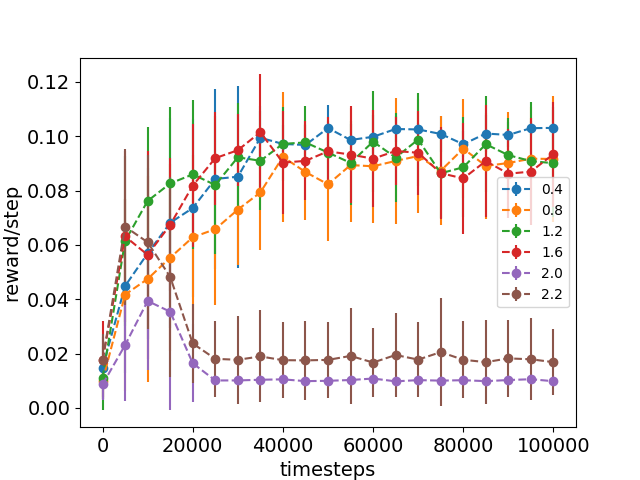
\includegraphics[width=\linewidth]{Study_2/2.4/visualizations/scores_filter_size.png}
      \caption{Learning curves for each size of filter}
  \end{subfigure}
  \begin{subfigure}[b]{0.4\linewidth}
    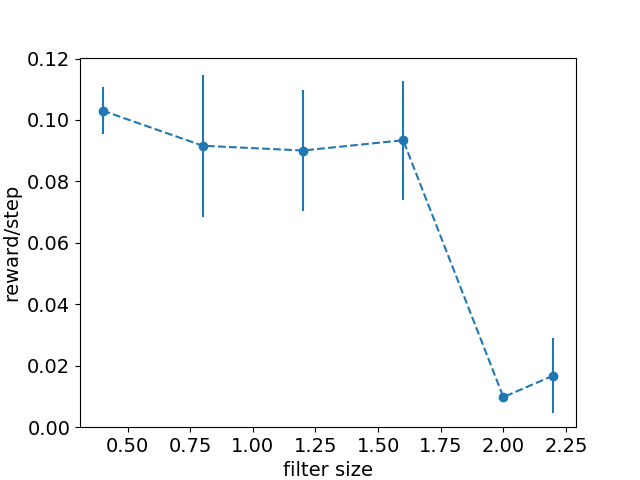
\includegraphics[width=\linewidth]{Study_2/2.4/visualizations/total_scores.png}
    \caption{final score according to the filter size}
  \end{subfigure}
   \caption{corner filter with random walk exploration}
    \label{fig:corner_curves_random_walk}
\end{figure}

The same performance drop is clearly present in Figure  \ref{fig:corner_curves_random_walk}, with the 2.0 and 2.2 radius filters.

\begin{figure}[H]
  \centering
   \begin{subfigure}[b]{0.3\linewidth}
    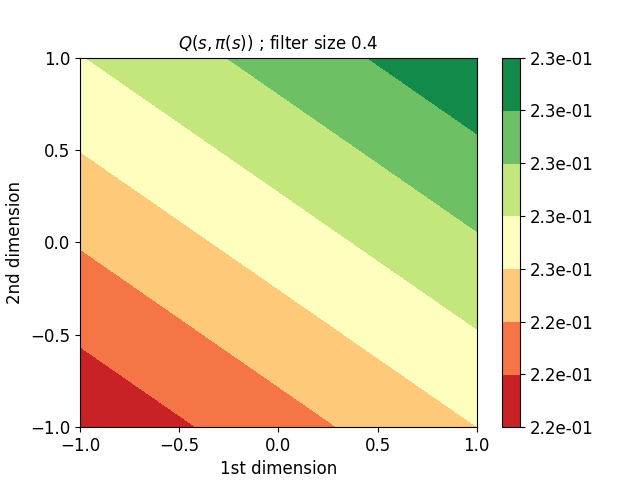
\includegraphics[width=\linewidth]{Study_2/2.4/visualizations/Q_contour_0_4.png}
      \caption{0.4 radius $Q(s, \Pi(s))$}
  \end{subfigure}
   \begin{subfigure}[b]{0.3\linewidth}
    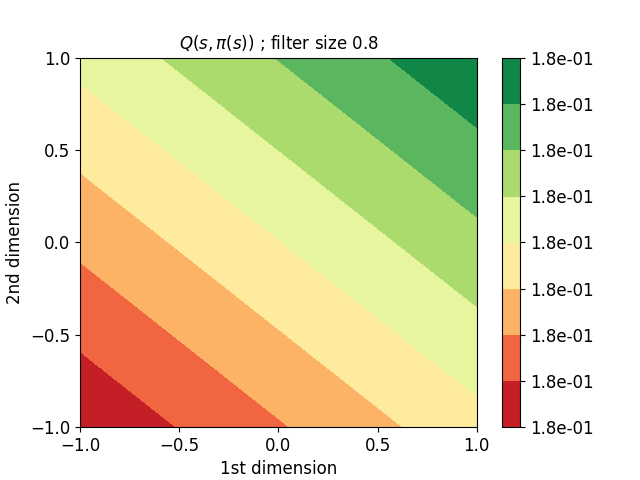
\includegraphics[width=\linewidth]{Study_2/2.4/visualizations/Q_contour_0_8.png}
      \caption{0.8 radius $Q(s, \Pi(s))$}
  \end{subfigure}
   \begin{subfigure}[b]{0.3\linewidth}
    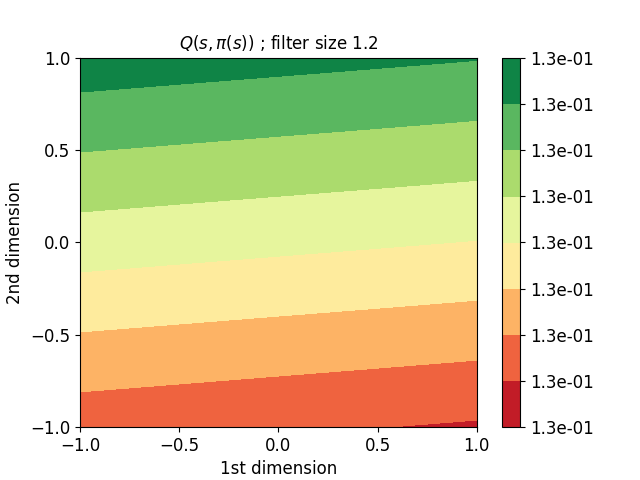
\includegraphics[width=\linewidth]{Study_2/2.4/visualizations/Q_contour_1_2.png}
      \caption{1.2 radius $Q(s, \Pi(s))$}
  \end{subfigure}
   \begin{subfigure}[b]{0.3\linewidth}
    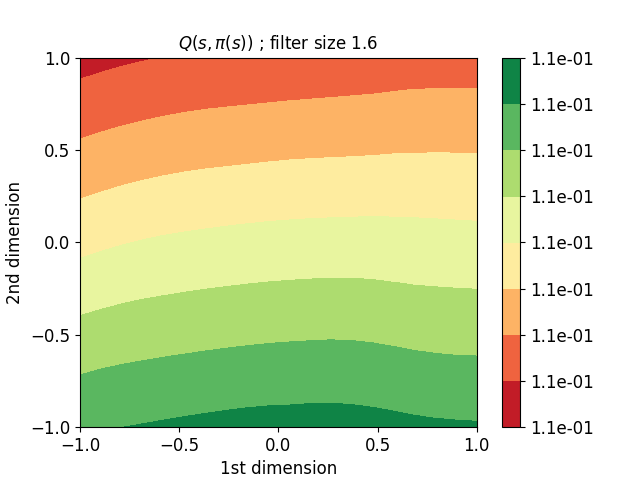
\includegraphics[width=\linewidth]{Study_2/2.4/visualizations/Q_contour_1_6.png}
      \caption{1.6 radius $Q(s, \Pi(s))$}
  \end{subfigure}
   \begin{subfigure}[b]{0.3\linewidth}
    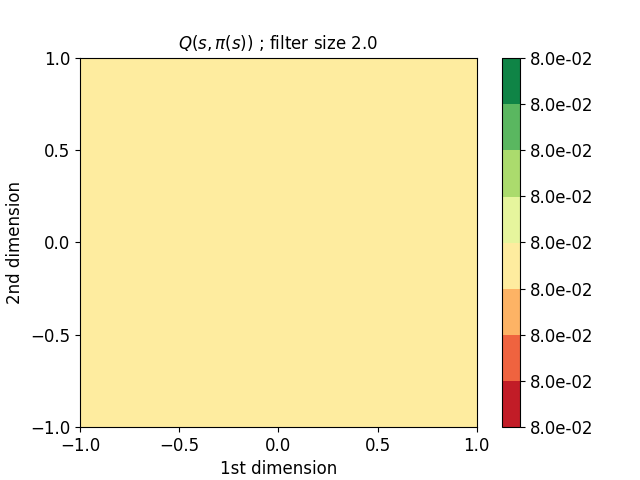
\includegraphics[width=\linewidth]{Study_2/2.4/visualizations/Q_contour_2_0.png}
      \caption{2.0 radius $Q(s, \Pi(s))$}
  \end{subfigure}
    \begin{subfigure}[b]{0.3\linewidth}
    \includegraphics[width=\linewidth]{Study_2/2.4/visualizations/Q_contour_2_2.png}
      \caption{2.2 radius $Q(s, \Pi(s))$}
  \end{subfigure}
  \caption{Sample policies : corner filter with random walk exploration}
  \label{fig:corner_contour_random_walk}
\end{figure}

 As we can see in Figure \ref{fig:corner_contour_random_walk} the policy is impacted earlier, around 1.2 a shift is noticeable. The sized above increase that effect and when the 2.0 radius is used we start noticing that the Q values estimations are vanishing as in the previous study.
 
 \begin{figure}[H]
  \centering
  \begin{subfigure}[b]{0.3\linewidth}
    \includegraphics[width=\linewidth]{Study_2/2.4/visualizations/Pi_arrow_1_6.png}
      \caption{1.6 radius $\Pi(s)$}
  \end{subfigure}
   \begin{subfigure}[b]{0.3\linewidth}
    \includegraphics[width=\linewidth]{Study_2/2.4/visualizations/Pi_arrow_2_0.png}
      \caption{2.0 radius $\Pi(s)$}
  \end{subfigure}
   \begin{subfigure}[b]{0.3\linewidth}
    \includegraphics[width=\linewidth]{Study_2/2.4/visualizations/Pi_arrow_2_2.png}
      \caption{2.2 radius $\Pi(s)$}
  \end{subfigure}
  \caption{Sample policies : 1.6, 2.0 and 2.2 radius}
  \label{fig:sample_policies_corner_sequential}
  \end{figure}
 
 In Figure \ref{fig:sample_policies_corner_sequential} the 1.6 radius filter visualizations show again a gap between the Actor and the Critic representation of the observation space. On the 2.0 and 2.2 filter size have their actions directed to the bottom left corner where only the low reward is present which explains the lower score. Those approximations errors might be reduced by using an algorithm reducing the approximations errors such as TD3 \cite{fujimoto_addressing_2018}.
 
\subsection{Study 3: Number of dimensions of the environement}

In this study we analyze the influence of the number of dimensions in the environment on the overall performances of DDPG.

\subsubsection{High and low rewards on each dimension}

We test the hypothesis which would be that the more dimensions there are in the environment more it is difficult for a DDPG agent to learn something form the environment. This test runs in environments with high and low rewards on each dimensions, as in Figure \ref{fig:1d_env} and Figure \ref{fig:2d_2_env}, from environment with 1 dimensions to environment with 4096 dimensions.

Parameters for this experiment:
\begin{itemize}
    \item[] \lstinline|--dimensions=| $2^0, 2^2, 2^4, 2^6, 2^8, 2^{10}, 2^{12}, 2^{14}$
    \item[] \lstinline|--learning_timesteps=5k|
    \item[] \lstinline|--eval_freq=250|
    \item[] \lstinline|--exploration_timesteps=32k|
    \item[] \lstinline|--exploration_mode="uniform"|
    \item[] \lstinline|--buffer_size=32k|
    \item[] \lstinline|--speed_limit_mode="vector_norm"|
\end{itemize}

\begin{figure}[H]
  \centering
  \begin{subfigure}[b]{0.45\linewidth}
    \includegraphics[width=\linewidth]{Study_3/half_norm/scores_dimensions.png}
      \caption{Learning curves for each number of dimensions}
  \end{subfigure}
  \begin{subfigure}[b]{0.45\linewidth}
    \includegraphics[width=\linewidth]{Study_3/half_norm/total_scores.png}
    \caption{Final score according to the numbers of dimensions}
  \end{subfigure}
  \caption{Scores according to the number of dimensions with half low rewards and half high rewards}
  \label{fig:curves_dimensions_half_norm}
\end{figure}

The results shown in Figure \ref{fig:curves_dimensions_half_norm} do not enable us to validate our hypothesis because the agent seems not to have learned anything for any number of dimensions, it just seems to be much more efficient with high dimensional environments. Surprisingly the score increases with the number of dimensions. After reflection it seems like it can be explained by the structure of the environment and the way the agent is initially located in it. At the beginning of each epoch the agent appears at a random position in the environment on each dimensions, so the more dimensions there are the more likely the agent will appear near at least one face of the hypercube, such way that it has to move just few steps to reach the reward. When the number of dimensions tends to infinity the agent always appears at a distance of one step from at least one high reward which explains the result of Figure \ref{fig:curves_dimensions_half_norm} which shows that the average reward per step tends to one when the number of dimensions tends to infinity.

\subsubsection{High and low rewards on each dimension with the respawn position centered in the environment}

In order verify this interpretation we decided conduct a counter experiment where the agent appears only in the center of the environment. The goal of this experiment is to make sure that increasing the number of dimension will not lead to increase the probability for the agent to appear near an edge. And to really see the influence of the number of dimension of the learning ability of DDPG. So in this experiment we run exactly the same experiment as before except that we introduced a parameter to fix the starting position at the center of the environment.

Parameters for this experiment:
\begin{itemize}
    \item[] \lstinline|--dimensions=| $2^0, 2^2, 2^4, 2^6, 2^8, 2^{10}$
    \item[] \lstinline|--learning_timesteps=5k|
    \item[] \lstinline|--eval_freq=250|
    \item[] \lstinline|--exploration_timesteps=32k|
    \item[] \lstinline|--exploration_mode="uniform"|
    \item[] \lstinline|--buffer_size=32k|
    \item[] \lstinline|--speed_limit_mode="vector_norm"|
    \item[] \lstinline|--reset_radius=0|
\end{itemize}

\begin{figure}[H]
  \centering
  \begin{subfigure}[b]{0.45\linewidth}
    \includegraphics[width=\linewidth]{Study_3/half_reset_norm/scores_dimensions.png}
      \caption{Learning curves for each number of dimensions}
  \end{subfigure}
  \begin{subfigure}[b]{0.47\linewidth}
    \includegraphics[width=\linewidth]{Study_3/half_reset_norm/total_scores.png}
    \caption{Final score according to the numbers of dimensions}
  \end{subfigure}
  \caption{Scores according to the number of dimensions with half low rewards and half high rewards}
  \label{fig:curves_dimensions_half_reset_norm}
\end{figure}

Now the result shown in Figure \ref{fig:curves_dimensions_half_reset_norm} is slightly different, we can see that for each number of dimensions the agent starts with approximately the same score. It seems like our interpretation of the previous experiment was probably true because our modification in the parameters had the desired effect. We see here that when the number or dimensions increases the scores reduces. That's what we expected a the beginning of this study, and it is probably because the agent starting for the center of the environment try to move in all the dimensions, and since its velocity vector norm is limited, if it move in all the dimensions simultaneously it will move very slowly on each dimension and then never found any reward which are at the extremities of the environment on each dimension.

\subsubsection{High and low rewards on each dimension with the respawn position centered in the environment and independent actions}

In order to verify if our previous interpretation is right we run the same test as before, except that now the actions are independent the one from each other, meaning that if the agent move in all directions at the same time it will move on each direction at the speed it want, its velocity vector norm is not bounded the agent just has a max velocity on each direction. With this modification if our prediction are right, the performance of DDPG should not decrease while the number of dimensions increases, because by moving on each dimension as if the environment has a single dimension, the agent would find the rewards as easily.

Parameters for this experiment:
\begin{itemize}
    \item[] \lstinline|--dimensions=| $2^0, 2^1, 2^2, 2^3, 2^4, 2^5, 2^6, 2^7$
    \item[] \lstinline|--learning_timesteps=5k|
    \item[] \lstinline|--eval_freq=250|
    \item[] \lstinline|--exploration_timesteps=32k|
    \item[] \lstinline|--exploration_mode="uniform"|
    \item[] \lstinline|--buffer_size=32k|
    \item[] \lstinline|--speed_limit_mode="independent"|
    \item[] \lstinline|--reset_radius=0|
\end{itemize}

\begin{figure}[H]
  \centering
  \begin{subfigure}[b]{0.45\linewidth}
    \includegraphics[width=\linewidth]{Study_3/half_reset_indept/scores_dimensions.png}
      \caption{Learning curves for each number of dimensions}
  \end{subfigure}
  \begin{subfigure}[b]{0.47\linewidth}
    \includegraphics[width=\linewidth]{Study_3/half_reset_indept/total_scores.png}
    \caption{Final score according to the numbers of dimensions}
  \end{subfigure}
  \caption{Scores according to the number of dimensions with half low rewards and half high rewards}
  \label{fig:curves_dimensions_half_reset_indept}
\end{figure}

In Figure \ref{fig:curves_dimensions_half_reset_indept} we can see that the convergence rate seems to increase with the number of dimensions, and the standard deviation decreases. This can be explained by the fact that the agent is now free to explore all the dimensions independently, the more dimensions there are faster the agent will reach a high reward on at least one dimension. The gradient towards this dimension will increase so that it can be exploited. As the process repeats and the number of dimensions increases, the number of dimensions that can be exploited also increases improving the convergence rate, this gives the agent more axis of movement towards a high reward. As there are $n/2$ high reward, with an increasing n, the agent expected time to reach a high rewards is stabilized which leads to very low standard deviation.

We saw that seems to converge for each number of dimensions in this configuration, so we want now to compare the convergence time needed to reach the optimal policy according to the number of dimensions. The agent appears at the center of the environment which is at a minimum distance of 1 form the edges of the hypercube and the maximum velocity of the agent is set to 0.1 on each dimension, so if the agent learns the optimal policy its score would be of 1 reward each 10 steps, which means a reward per step of 0.1. To compare the convergence of DDPG on the different size on environment we consider that a policy is optimal when the agent reach a an average score of $0.8$ rewards per step. 
 
\begin{figure}[H]
  \centering
  \includegraphics[width=0.5\linewidth]{Study_3/half_convergence_reset_indept/convergences.png}
  \caption{Convergence time according to the number of dimensions}
  \label{fig:convergence}
  \vspace{2cm}
\end{figure}

Figure \ref{fig:convergence} shows that the average timesteps needed to reach the optimal policy seems to decrease linearly while the number of dimensions increases.

\subsubsection{High and low rewards on the first dimension only, with the respawn position centered in the environment and independent actions}

This study is the same as the previous one, except that we put only one high and low reward on the first dimension, and all the other dimensions does not contains any rewards. For example this two environments Figure \ref{fig:1d_env} and Figure \ref{fig:2d_1_env} respects this constraint. We decided to do this study to verify if the result of previous study is due to the fact that the number of rewards increases with the number of dimensions. We will see if a lot of dimensions and only rewards on the first dimension makes the learning harder or not.

Parameters for this experiment:
\begin{itemize}
    \item[] \lstinline|--dimensions=| $2^0, 2^1, 2^2, 2^3, 2^4, 2^5, 2^6, 2^7$
    \item[] \lstinline|--learning_timesteps=5k|
    \item[] \lstinline|--eval_freq=250|
    \item[] \lstinline|--exploration_timesteps=32k|
    \item[] \lstinline|--exploration_mode="uniform"|
    \item[] \lstinline|--buffer_size=32k|
    \item[] \lstinline|--speed_limit_mode="independent"|
    \item[] \lstinline|--reset_radius=0|
    \item[] \lstinline|--high_reward_count="one"|
    \item[] \lstinline|--low_reward_count="one"|
\end{itemize}

\begin{figure}[H]
  \centering
  \begin{subfigure}[b]{0.45\linewidth}
    \includegraphics[width=\linewidth]{Study_3/one_reset_indept/scores_dimensions.png}
      \caption{Learning curves for each number of dimensions}
  \end{subfigure}
  \begin{subfigure}[b]{0.47\linewidth}
    \includegraphics[width=\linewidth]{Study_3/one_reset_indept/total_scores.png}
    \caption{Final score according to the numbers of dimensions}
  \end{subfigure}
  \caption{Scores according to the number of dimensions with one low reward and one high reward}
  \label{fig:curves_dimensions_one}
\end{figure}

Figure \ref{fig:curves_dimensions_one} shows the performances achieved during the whole learning process per dimension. As we can see, the convergence rate seems to stay stable with the number of dimensions, but with a very high standard deviation. So it seems to mean that the number of dimensions does not affect the ability of DDPG to learn the policy on the important dimension. Since all the dimensions are independents, DDPG can rely only on the single rewarding dimension in order to achieve the highest rewarding goal.

\section{Conclusion}

\subsection{Results}

%study 1 2
We found a strong correlation between the size of the experience replay buffer and the learning ability of DDPG in case of batch learning on a fixed dataset, the simplicity of our environment make it also very easy to learn with a small replay buffer. But contrary to \cite{fujimoto_off-policy_2018}, we did not found that learning from a fixed dataset of experiences uncorrelated with the used policy leads to extrapolation errors. We just saw differences between data collection methods, learning from fixed dataset of experiences gathered by uniform exploration works much better than learning from experiences gathered by random walk, but when the size of the replay buffer increases, the differences between random walk and uniform sampling disappear.

%study2
When analysing the behaviour of DDPG on a filtered environment we did notice that DDPG's interpolations abilities are far superior to its extrapolation abilities. The centered filter was handled much better than the corner one. However, we did not notice the divergent behaviour that we were expecting as described in \cite{achiam_towards_2019}.
Additionaly, the exploration scheme seemed to have no impact whatsoever on the resulting performances.

%study3
The results of the study on the number of dimensions in the environment on the learning ability of DDPG taught us
more about the environment than about DDPG. The reason why DDPG is unable to learn on our high dimensional
environments is not due to DDPG itself bue to the structure of the environment where the actions of the agent are not
independent. The norm of the velocity vector being bounded by 1 if too many dimensions are used when taking an action the resulting actions on each dimensions will be negligible because of the normalisation step, therefore the agent won't make any progress. With independant actions this problem is no more and DDPG is able to learn faster and reach higher reward / step performances since it is able to combine its speed along several dimensions.

%linear learning problem

Over all the experiment we did on our environment, it seems that regardless of the dimensionality, exploration scheme or other parameters DDPG will always learn a linear action value function. This leads to the agent learning a linear policy that usually takes it towards the highest rewarding corner of the environment. This way might be the easiest to be guaranteed a high reward in the end but it is certainly not the fastest, especially not in high dimensional environments.
The behaviour we expected was to go straight to the closest high reward, focusing only on the dimension that matter in order to maximise the reward / step parameter.

\subsection{Future work}

%future work to resolve the linearity problem
Future work could be to try to solve the problem of the linear policy learned by DDPG, by trying bigger neural network  than the default ones or other activation functions than ReLu. Maybe the linear policy learned by DDPG is due to the fact that our environment provides only positives rewards whatever direction the agent chooses, then the ReLus could works like linear functions. So further experiments have to be conducted to understand why DDPG learns a linear policy instead of the optimal policy computed with the value iteration algorithm on the discretized environment. 

%after resolving this
After resolving the problem of linearity, with plenty of room for improvements and ideas of additional studies we are for instance looking to use Hindsight Experience Replay \cite{andrychowicz_hindsight_2017} on all the existing studies to analyze the possible performance improvements. Study 2 starts addressing some of the issues related to divergence on Q values approximation \cite{achiam_towards_2019} over a filtered space but different point of interest are also considered in order to validate the results exposed by the team from Deep Mind on the so called deadly Triad \cite{van_hasselt_deep_2018}.

Adding more complexity and configurability to the environment would also allow for deeper studies. By introducing a dependence between the different dimensions and more reward distribution patterns to further investigate the abilities and limits of DDPG.


\bibliographystyle{ieeetr}  
\bibliography{MyLibrary}

\end{document}
